\documentclass[letterpaper,12pt,titlepage,oneside,final]{book}

% For PDF, suitable for double-sided printing, change the PrintVersion variable below
% to "true" and use this \documentclass line instead of the one above:
%\documentclass[letterpaper,12pt,titlepage,openright,twoside,final]{book}

% Some LaTeX commands I define for my own nomenclature.
% If you have to, it's better to change nomenclature once here than in a 
% million places throughout your thesis!
\newcommand{\package}[1]{\textbf{#1}} % package names in bold text
\newcommand{\cmmd}[1]{\textbackslash\texttt{#1}} % command name in tt font 
\newcommand{\href}[1]{#1} % does nothing, but defines the command so the
% print-optimized version will ignore \href tags (redefined by hyperref pkg).
%\newcommand{\texorpdfstring}[2]{#1} % does nothing, but defines the command
% Anything defined here may be redefined by packages added below...

% This package allows if-then-else control structures.
\usepackage{ifthen}
\usepackage{listings}
\usepackage{color}

\definecolor{dkgreen}{rgb}{0,0.6,0}
\definecolor{gray}{rgb}{0.5,0.5,0.5}
\definecolor{mauve}{rgb}{0.58,0,0.82}

\lstset{frame=tb,
	language=Java,
	aboveskip=3mm,
	belowskip=3mm,
	showstringspaces=false,
	columns=flexible,
	basicstyle={\small\ttfamily},
	numbers=none,
	numberstyle=\tiny\color{gray},
	keywordstyle=\color{blue},
	commentstyle=\color{dkgreen},
	stringstyle=\color{mauve},
	breaklines=true,
	breakatwhitespace=true,
	tabsize=3
}
\newboolean{PrintVersion}
\setboolean{PrintVersion}{false} 
% CHANGE THIS VALUE TO "true" as necessary, to improve printed results for hard copies
% by overriding some options of the hyperref package below.

%\usepackage{nomencl} % For a nomenclature (optional; available from ctan.org)
\usepackage{amsmath,amssymb,amstext} % Lots of math symbols and environments
\usepackage[pdftex]{graphicx} % For including graphics N.B. pdftex graphics driver 
\usepackage[acronym,automake]{glossaries}
\usepackage{siunitx}
\usepackage{multirow}
\usepackage{setspace}
\usepackage[paper=a4paper,margin=1in]{geometry}
\usepackage{tikz}

%here declear the acronym
\newacronym{who}{WHO}{World Health Organization}
\newacronym{ncoa}{NCOA}{the National Council of Aging}
\newacronym{mems}{MEMS}{Micro-Electro-Mechanical}
\newacronym{imu}{IMU}{Inertia Measurement Unit}
\newacronym{adc}{ADC}{analog-to-digital converter}
\newacronym{lsb}{LSB}{Least Significant Bit}
\newacronym{ssf}{SSF}{Sensitivity Scale Factor}
\newacronym{mcu}{MCU}{Micro-Controller Unit}
\newacronym{iot}{IoT}{Internet-of-Things}
\newacronym{us}{U.S.}{United State of America}
\newacronym{adl}{ADLs}{Activity of Daily Living}

\makeglossaries
% Hyperlinks make it very easy to navigate an electronic document.
% In addition, this is where you should specify the thesis title
% and author as they appear in the properties of the PDF document.
% Use the "hyperref" package 
% N.B. HYPERREF MUST BE THE LAST PACKAGE LOADED; ADD ADDITIONAL PKGS ABOVE
\usepackage[pdftex,letterpaper=true,pagebackref=false]{hyperref} % with basic options
% N.B. pagebackref=true provides links back from the References to the body text. This can cause trouble for printing.
\hypersetup{
	plainpages=false,       % needed if Roman numbers in frontpages
	pdfpagelabels=true,     % adds page number as label in Acrobat's page count
	bookmarks=true,         % show bookmarks bar?
	unicode=false,          % non-Latin characters in Acrobat’s bookmarks
	pdftoolbar=true,        % show Acrobat’s toolbar?
	pdfmenubar=true,        % show Acrobat’s menu?
	pdffitwindow=false,     % window fit to page when opened
	pdfstartview={FitH},    % fits the width of the page to the window
	pdftitle={uWaterloo\ LaTeX\ Thesis\ Template},    % title: CHANGE THIS TEXT!
	%    pdfauthor={Author},    % author: CHANGE THIS TEXT! and uncomment this line
	%    pdfsubject={Subject},  % subject: CHANGE THIS TEXT! and uncomment this line
	%    pdfkeywords={keyword1} {key2} {key3}, % list of keywords, and uncomment this line if desired
	pdfnewwindow=true,      % links in new window
	colorlinks=true,        % false: boxed links; true: colored links
	linkcolor=black,         % color of internal links
	citecolor=black,        % color of links to bibliography
	filecolor=magenta,      % color of file links
	urlcolor=cyan           % color of external links
}
\ifthenelse{\boolean{PrintVersion}}{   % for improved print quality, change some hyperref options
	\hypersetup{	% override some previously defined hyperref options
		%    colorlinks,%
		citecolor=black,%
		filecolor=black,%
		linkcolor=black,%
		urlcolor=black}
}{} % end of ifthenelse (no else)

% Setting up the page margins...
% uWaterloo thesis requirements specify a minimum of 1 inch (72pt) margin at the
% top, bottom, and outside page edges and a 1.125 in. (81pt) gutter
% margin (on binding side). While this is not an issue for electronic
% viewing, a PDF may be printed, and so we have the same page layout for
% both printed and electronic versions, we leave the gutter margin in.
% Set margins to minimum permitted by uWaterloo thesis regulations:
\setlength{\marginparwidth}{0pt} % width of margin notes
% N.B. If margin notes are used, you must adjust \textwidth, \marginparwidth
% and \marginparsep so that the space left between the margin notes and page
% edge is less than 15 mm (0.6 in.)
\setlength{\marginparsep}{0pt} % width of space between body text and margin notes
\setlength{\evensidemargin}{0.125in} % Adds 1/8 in. to binding side of all 
% even-numbered pages when the "twoside" printing option is selected
\setlength{\oddsidemargin}{0.125in} % Adds 1/8 in. to the left of all pages
% when "oneside" printing is selected, and to the left of all odd-numbered
% pages when "twoside" printing is selected
\setlength{\textwidth}{6.375in} % assuming US letter paper (8.5 in. x 11 in.) and 
% side margins as above
\raggedbottom
\setcounter{tocdepth}{3}
\setcounter{secnumdepth}{3}
% The following statement specifies the amount of space between
% paragraphs. Other reasonable specifications are \bigskipamount and \smallskipamount.
\setlength{\parskip}{\medskipamount}

% The following statement controls the line spacing.  The default
% spacing corresponds to good typographic conventions and only slight
% changes (e.g., perhaps "1.2"), if any, should be made.
\renewcommand{\baselinestretch}{1} % this is the default line space setting

% By default, each chapter will start on a recto (right-hand side)
% page.  We also force each section of the front pages to start on 
% a recto page by inserting \cleardoublepage commands.
% In many cases, this will require that the verso page be
% blank and, while it should be counted, a page number should not be
% printed.  The following statements ensure a page number is not
% printed on an otherwise blank verso page.
\let\origdoublepage\cleardoublepage
\newcommand{\clearemptydoublepage}{%
	\clearpage{\pagestyle{empty}\origdoublepage}}
\let\cleardoublepage\clearemptydoublepage
%======================================================================5
%   L O G I C A L    D O C U M E N T -- the content of your thesis
%======================================================================
\begin{document}
%delete chapter 
\makeatletter
\def\@makechapterhead#1{%
	{\parindent \z@ \raggedright \normalfont
		\ifnum \c@secnumdepth >\m@ne
		\huge\bfseries \thechapter.\ % <-- Chapter # (without "Chapter")
		\fi
		\interlinepenalty\@M
		#1\par\nobreak% <------------------ Chapter title
		\vskip 10\p@% <------------------ Space between chapter title and first paragraph
}}
% For a large document, it is a good idea to divide your thesis
% into several files, each one containing one chapter.
% To illustrate this idea, the "front pages" (i.e., title page,
% declaration, borrowers' page, abstract, acknowledgements,
% dedication,   of contents, list of tables, list of figures,
% nomenclature) are contained within the file "uw-ethesis-frontpgs.tex" which is
% included into the document by the following statement.
%----------------------------------------------------------------------
% FRONT MATERIAL
%----------------------------------------------------------------------
% T I T L E   P A G E
% -------------------
% Last updated May 24, 2011, by Stephen Carr, IST-Client Services
% The title page is counted as page `i' but we need to suppress the
% page number.  We also don't want any headers or footers.
\pagestyle{empty}
\pagenumbering{roman}

% The contents of the title page are specified in the "titlepage"
% environment.	
\begin{titlepage}
		% Side by side figure
		\begin{figure}
			\begin{minipage}[c]{0.4\linewidth}
			
\includegraphics[scale=0.3]{VGU}
			\end{minipage}
			\hfil
				\begin{minipage}[c]{0.2\linewidth}
				
\includegraphics[scale=0.25]{FRAUAS}
			\end{minipage}	
		\end{figure}
     	%Text front page
     
        \begin{center}
        \normalsize
        	Frankfurt University of Applied Science\\
        	Department 2: Computer Science and Engineering\\
        	\vspace*{0.1cm}
        	Vietnamese - German University\\
        	Department of Electrical Engineering and Infomation Technology
        \vspace*{1cm}	
        \begin{center}
        	Bachelor Thesis
        \end{center}
        \vspace*{1.3cm}
        \Large
        {\bf DESIGN AND IMPLENTATION OF A WIRELESS FALL DETECTION NETWORK PROTOTYPE USING MEMS SENSORS}

        \vspace*{0.5cm}

        \normalsize
        by \\

        \vspace*{0.5cm}

        \Large
        Ho Ngoc Khang Minh \\
      	\normalsize
      	\vspace{0.2cm}
		Matriculation No.: 1148602
		
        \vspace*{1.5cm}
        \large
       	First Supervisor: Prof. Dr.-Ing. Kira Kastell \\
       	Second Supervisor: Dipl. -Ing Mohammad Reza Mansooji \\
       	\vspace{1.7cm}
        \normalsize
        Submitted in partial fulfillment of the requirements\\
        for the degree of Bachelor Engineering in study program\\
        Electrical Engineering \& Information Technology,\\
        Vietnamese - German University

        \vspace*{3.0cm}
		
        Frankfurt am Main, Germany 2018 \\
	
        
        \end{center}
\end{titlepage}

% The rest of the front pages should contain no headers and be numbered using Roman numerals starting with `ii'
\pagestyle{plain}
\setcounter{page}{2}
\cleardoublepage
 % Ends the current page and causes all figures and tables that have so far appeared in the input to be printed.
% In a two-sided printing style, it also makes the next page a right-hand (odd-numbered) page, producing a blank page if necessary.
 


% D E C L A R A T I O N   P A G E
% -------------------------------
  % The following is the sample Delaration Page as provided by the GSO
  % December 13th, 2006.  It is designed for an electronic thesis.
  
  {
  	\begin{center}
  		\Large
  		\bf Disclamer
  	\end{center}
  	{
  		\setstretch{1.5}
  		\par
  		I hereby declare that this thesis is a product of my own work, unless otherwise
  		referenced. I also declare that all opinions, results, conclusions and recommendations are
  		my own and may not represent the policies or opinions of Vietnamese - German University and Frankfurt University of Applied Science. \par
  	}
  	\vspace{3cm}
  	\hspace{11cm}
  	Ho Ngoc Khang Minh
  	\cleardoublepage
  }	

\cleardoublepage

\pagestyle{plain}
\setcounter{page}{3}

\cleardoublepage % Ends the current page and causes all figures and tables that have so far appeared in the input to be printed.
% In a two-sided printing style, it also makes the next page a right-hand (odd-numbered) page, producing a blank page if necessary.

\begin{center}
\vspace*{\fill}
\copyright 2018 by Ngoc Khang Minh, Ho. All right reserved.
\vspace*{\fill}
\end{center}



\cleardoublepage
%\newpage

% A B S T R A C T
% ---------------
\begin{center}\textbf{Abstract}\end{center}
{
	\setstretch{1.5}
	\par
	Falling is becoming a serious problem to elderly people, often causing unpredictable injuries such as hip fractures, head traumas, etc. More seriously, falls may lead to disability or even death on the victim if assistances from caregivers are not received in time. From this situation, there is a need for a wireless communication network which can automatically detect the fall and send an alarm to the caregivers if there is no safe signal from the victim within 10 minutes. There have been several algorithms such as detection of body orientation after a fall, image processing to detect the fall or applying machine learning techniques (Support Vector Machine (SVM), Markov model) in classifying between falling and other activities of daily living (ADL). However, these complex techniques require a huge amount of computations which can result in the system being overloaded or heavily delayed.\par
	Addressing this problem calls for less computation-intensive techniques while retaining the accuracy and robustness of the system. One such approach is the combination of data from both accelerometer and gyroscope. The focus of this thesis is developing a wireless fall detection network which can combine the data from the above sensors to detect falls and distinguish them from fall-like activities. A comparison on the performance of this network with other existing works is also included to evaluate the robustness of the system.\par
	\vspace{1cm}
	\textit{\textbf{Keywords:} elderly people, fall detection, accelerometer, gyroscope,  wireless communication network}
}
\cleardoublepage
%\newpage

% A C K N O W L E D G E M E N T S
% -------------------------------
\begin{center}\textbf{Acknowledgements}\end{center}
{
	\setstretch{1.5}
	\par
	I would like to express my sincere appreciation to Prof. Dr.-Ing. Kira Kastell, Vice President of Frankfurt University of Applied Science (FRA-UAS) for supervising, supporting and encouraging me during the time I conduct my senior project and final thesis. Also, I would like to thank Mr. Dipl.-Ing Mansooji - communication lab engineer at FRA-UAS, Dr. Vo Bich Hien - lecturer and Mr. Duong Huynh Bao - former control lab engineer at Vietnamese - German University for guiding me on technical and programming aspects. I also would like to thank my family for their supports during my bachelor degree time. This project would not be completed without their grateful guidances and supports. Thanks to their encouragements, I can improve myself, not only on the fundamental background in my major, but also necessary skills for my future career. I would like to mention all of my seniors and classmates who have helped me through this thesis.\par
	\vspace{1cm}
}
\cleardoublepage

%\newpage

% D E D I C A T I O N
% -------------------
%\newpage

% T A B L E   O F   C O N T E N T S
% ---------------------------------
\renewcommand\contentsname{Table of Contents}
\tableofcontents
\cleardoublepage
\phantomsection
%\newpage

% L I S T   O F   T A B L E S
% ---------------------------
\addcontentsline{toc}{chapter}{List of Tables}
\listoftables
\cleardoublepage
\phantomsection		% allows hyperref to link to the correct page
%\newpage

% L I S T   O F   F I G U R E S
% -----------------------------
\addcontentsline{toc}{chapter}{List of Figures}
\listoffigures
\cleardoublepage
\phantomsection		% allows hyperref to link to the correct page
%\newpage

%Acronym section%

% L I S T   O F   S Y M B O L S
% -----------------------------
% To include a Nomenclature section
% \addcontentsline{toc}{chapter}{\textbf{Nomenclature}}
% \renewcommand{\nomname}{Nomenclature}
% \printglossary
% \cleardoublepage
% \phantomsection % allows hyperref to link to the correct page
% \newpage

% Change page numbering back to Arabic numerals
\pagenumbering{arabic}

 
\printglossaries
\setstretch{1.5}
%----------------------------------------------------------------------
% MAIN BODY
%----------------------------------------------------------------------
% Because this is a short document, and to reduce the number of files
% needed for this template, the chapters are not separate
% documents as suggested above, but you get the idea. If they were
% separate documents, they would each start with the \chapter command, i.e, 
% do not contain \documentclass or \begin{document} and \end{document} commands.
%======================================================================
\chapter{Introduction}
%======================================================================

%----------------------------------------------------------------------
\section{Introduction to Fall}
%---------------------------------------------------------------------
Nowadays, falling is becoming a dangerous issue which mostly causes injuries and even disability or fatal death on humans, especially the elderly. According to Hwang \textit{et.at.} \cite{static1}, in the United States, one-third to one-half of elderly people over 65 years old fall at least one time each year  and two-third of them will do so again within the next 6 months. Every 11 seconds, there is an elderly person be treated in the hospital's emergency area due to fall-related injuries and every 19 minutes, one faller dies \cite{ncoa}. It is also reported that one out of every 200 falls results in a hip fracture on people with age among 65 and 69, increasing to one out of 10 for those aged 85 and more \cite{hip_fracture}. The most profound effect of falling is the loss of functioning associated with the dependency of the elderly for the rest of their life. Besides, a great amount of time and money have been spent on the medical treatments for the falls. Approximately \$179 million were used as direct medical costs for treating fatal falls and \$19 billion for non-fatal fall injuries within 2000 \cite{cost_fatal}.

\section{Definition of a Fall}
Before starting a research about falls, it is necessary to understand about the meaning of the term \textit{falls}. According to the \gls{who}, a fall is defined as an event which results in a person coming to rest inadvertently on the ground or floor or other lower level with or without loss of consciousness or injury \cite{who}. 

\section{Cause of a Fall}
In recent years, a lot of researches have been carried out by different groups to find out the causes of falls. There have been different ways to classify the causes of a fall such as age and sex, drugs, cognitive functions, postural control, etc. However, falling is an unintentional action, many causes usually combine to produce a fall. Therefore, these causes can be divided into two main categories, intrinsic and extrinsic, to ease the complexity of research activities.
\subsection{Intrinsic risk factors}
Intrinsic factors are the factors within the body. It is also the physical aspect of the body that can cause injuries. Intrinsic factors include physical diseases such as cognitive impairment, postural hypotension, cardiovascular problems, etc.\par
\vspace{0.3cm}
\textbf{\textit{Cognitive Impairment}}\par
It is well recognized that cognitive impairment is the most common cause of falls on humans, especially the elderly. Due to the research of Prudheim \textit{et al.} \cite{cognitive_1} in 1981, fallers have in general been found to have a higher prevalence of cognitive impairment than non-fallers. It is also reported that humans with dementia are approximately 3 times more likely to fall than non-demented \cite{cognitive_2}. The reason why patients with cognitive impairment are likely to fall is that they have increased reaction time, increased postural sway and increased leaning balance which result in the decrease of muscle strength, worse balance and poorer mobility. \par
\vspace{0.3cm}
\textbf{\textit{Postural Control}}\par
Postural control is a complex motor skill that requires the interaction of multiple body systems, which results in the ability to maintain postural orientation or postural stability \cite{postural_1}, \cite{postural_2}. The impairment of postural control is indicated as one of significant causes of the fall during any activity at any age. Impaired control of gait and balance are two main aspects of the postural control that have been considered in many studies about falls recently. Subjectively assessed gait has been reported to be abnormal in many fall activities, and other studies using more objective measurements have found some relations between the impaired gait and balance and risk of falling \cite{bibli_book}.

\vspace{0.3cm}
\textbf{\textit{Cardiovascular problem}}\par
Cardiovascular disorders are responsible for approximately 77\% of patients with unexplained or recurrent falls associated with loss of consciousness \cite{cardio_1}. The most common cardiac disorders linked to falls are carotid sinus syndrome, postprandial hypotension, orthostatic hypotension, vasovagal syncope, and bradyarrhythmias \cite{cause_cardio}. There is a fact that fallers with cardiovascular disorders have a greater mortality than those with non-cardiovascular or unknown causes \cite{cardio_2}.   
\subsection{Extrinsic risk factors}
Extrinsic factors are those related to the environment such as lighting, walking surface, loose carpets, and high or narrow steps. 

\vspace{0.3cm}
\textbf{\textit{Dim lighting or glare}}\par
Dim lighting is one significant cause of fall on humans, especially on the elderly. While walking in the low light condition, the patient's visibility is reduced which prevents them from detecting the obstacles on the walking path, hence causing stumble and fall. Too bright lighting can also cause fall on humans because of creating glares and distorting the way object look. \par
\vspace{0.3cm}
\textbf{\textit{Bad staircase design}}\par

Bad staircase design is also another extrinsic risk that causes the fall on humans. Too high or too low rise of staircases have caused a number of falls because people fail to perceive the abnormal elevation change or incur a misstep on descent. Besides, slippery surface of the treads can cause strip on patients while walking up or down the stairs. One more mistake of staircase design that can lead to the fall is lighting condition on the stair. Poor visibility and inadequate lighting can cause a user to misread the stair edge, resulting in faulty foot placement and falls.
\section{Consequence of Falls}
The consequences of falls are serious to humans at any age in any circumstance, but to the elderly, they have significance beyond that in younger people. There are different consequences related to the falls on humans including physical effects, psychological effects and other consequences such as dependency, hospital admission or economic consequences. 

\vspace{0.3cm}
\textbf{\textit{Physical consequences}}\par

Physical consequences of falls are always a significant aspect that many scientists have focused on in recent years. According to the \gls{ncoa} of the U.S., falls are the leading cause of fatal injuries and the most common cause of non-fatal traumas \cite{ncoa}. There are several physical injuries such as bruise, fracture or head injury reported to happen with patients who suffer from falls. In such injuries, hip fractures and head traumas are two common problems which are usually analyzed by researchers. \par
Hip fractures cause the greatest health problems and greatest number of death. It is reported that a quarter million hip fractures occur each year among people older than 50 years old in the U.S. but more common in women than men and increase in frequency with increasing age \cite{bibli_book}, \cite{medicinenet_fracture}. Most patients with the hip fractures after falls are hospitalized, but about half of them cannot return home or live independently after that. In 1986, it costs for more than \$3 billions for direct medical treatment of hip fractures \cite{medicinenet_fracture}.\par 

Head injuries also usually happen to patients after suffering a fall. It is reported that people with the age of over 65 years old make up for 10-15\% of admission to the hospital because of head injuries while three-quarters of them are caused by fall \cite{bibli_book}. In California from 1996 to 1999, 71\% of fall-related head injuries occurred in adults aged 65 and more \cite{head_injury_1}. The head trauma from a previous fall can increase the risk of repeated fall and head injuries in the near future.  \par

Finally, the most serious impact of fall is fatal injuries causing death to a patient. According to data from the \gls{who}, the fall morality rate of people with the age of over 65 in the \gls{us} (in 2003) was 36.8 per 100 000 citizens \cite{death_in_USA}. The main reason of these accidental death is that many patients had lied on the ground for several hours before receiving the help from caregivers. \par

\vspace{0.3cm}
\textbf{\textit{Psychological consequences}}\par
Fall can result in long lasting psychological impact, called fear of falling again, more than just short-term injuries. Those people who have fallen one time before seem to have a feeling of vulnerability which limits them from their normal activities. They may be worried about falling and hurting themselves again, thus stop going out on their own or reduce their level of physical activities. Unfortunately, in attempting to reduce their risk of falling,  they may increase the risk of falling because of the attenuation of physical functions and mobility. 	
\cleardoublepage
\vspace{0.3cm}
\textbf{\textit{Other consequences}}\par
Some research indicated that there are other consequences such as dependency, hospital admission or economic consequence. As already mentioned, the fear of falling again prevents patients from living alone and starting depending on the long-term nursing care. This consequence directly leads to increased dependency, which requires more time and financial resources from both government and family. \par
Falls are also the main reason for people to be admitted to hospital as an emergency case. Due to the information provided by the Accident Department at a sample of hospitals in England and Wales, in 1998, approximately 200 000 people over 60 are treated at this hospital per year because of a fall at home \cite{other_consequence_1}.\par
Finally, falls are also an economic burden of every country around the world, especially for low and lower middle countries. According to the U.S. Center for Disease Control and Prevention, in 2015, there was \$50 billion being used for fall injuries and expected to increase as the population ages and may reach \$67.7 billion by 2020 \cite{ncoa}. These costs are spent for hospitalization, medical, pharmaceutical, nursing home and other costs which are related to the medical treatments for fall patients.

\section{Challenges in Detecting Falls}
As mentioned in the previous section, most of patient's death is caused by the late assistance from the caregivers after fall accidents. Timely detection can minimize the negative impacts of falls on patients. However, depending on age and physical condition, different people have different gaits, different balance ability that result in several types of fall. These falls can happen in any direction at any speed. Therefore, it is still a challenge to design a system which can detect successfully all the falls of patients. \par
Another challenge in detecting the fall is that it is difficult for a system to distinguish a real fall from other fall-liked activities such as sitting, jumping or running, which also result in high acceleration. Therefore, it is required to collect data from different subjects; and then, there should be some analyses to find out the most common pattern of every fall. From that, researchers can design an algorithm to detect the falls based on this pattern. However, it is not easy to collect data for the system from the daily life on real human bodies, since it is an accidental, dangerous action which can happen randomly at any time. Therefore, it is a overwhelming task for researchers to built a dataset for their system. 

\section{Objectives}
From the above challenges, it is necessary to study and design a wireless sensor network which can automatically detect the fall of a patient and send an alarm to the caregivers instantly to reduce their time of arrival, and hence reduce the mortality rate. The sensor node is portable and attached to the chest of the user. According to research of Gjoreski \textit{et al.} \cite{sensor_position1}, chest and waist are the most common places to put the sensor in fall detection system. Beside that, Huynh \textit{et al.} \cite{optimum_sensor_place} also determined chest as the optimal location for the sensor node. In addition, wearing such small device on the chest would cause no discomfort on user in their daily activities. This sensor node contains one accelerometer and one gyroscope to provide information about the body's acceleration and angular velocity during the fall event. This sensor node can connect to the host computer via Wi-Fi with the help of a Wi-Fi module called ESP8266 from ESPRESSIF\textregistered company and send data directly to a monitoring software on the computer. Upon detecting a fall, the sensor node will wait for the safe signal from the patient within the next 10 minutes. If there is no response, an emergency email will be sent immediately to the caregiver. There is also a super bright red led on the sensor node to indicate the fall that helps the caregiver to easily find out the patient. 
\section{Thesis Organization}
In chapter 1, basic knowledge about falls as well as the causes and consequences of them are introduced. It also provides the information about current challenges in detecting the fall and the motivation for this thesis. In chapter 2, a review of existing commercial fall detection devices on the market and researches related to this topic from  other research groups is included. Chapter 3 describes the problem of fall detection and a method to solve this problem. Also included in this chapter is the description of the algorithm used in this thesis. Chapter 4 describes the system with both hardware and software perspectives. Chapter 5 and 6 describe the data collection and analysis procedure as well as the result assessment of the experiments on a real human body. Finally, chapter 7 gives the conclusion for this thesis, the limitation of the current solution and recommendations for future works.
%======================================================================
\chapter{Literature Review}
Nowadays, there are a lot of companies focusing on developing portable fall detection devices to suffice the need of the current society where there are more and more elderly people falling every day. These products are used widely by many people around the world and have positive effects on health-care systems of the corresponding countries. Beside that, numerous universities and research groups carried out studies on the topic of fall detection from various perspectives and have great contributions to the evolution of health monitoring services.  
\section{Existing Commercial Devices}
One popular fall detection device, which is highly evaluated by customers, is the Medical Fall Alert in the \textit{Home Guardian} option from Medical Guardian. It is designed in form of a lightweight wearable neck pendant. This pendant is waterproof and small enough that it has no disturbance on the user's daily activity. Medical Guadian provides a home system including one base unit connecting to the monitoring station through landline and one auto-alert pendant on the user's body. Whenever detecting a fall, the wearable pendant will send a signal to the base unit and the base station will announce \textit{"Fall Detected, Press or Hold Button to Cancel"}. If the patient actually needs help, he(she) does not press the button. Then, the system will connect to operators at the monitoring center, they will ask if the patient needs help or not. If the patient cannot speak because of unconsciousness, the operators will automatically send emergency services to the patient's home. The monthly fee for this service is around \$44.95 per month and it is used inside the \gls{us}.

 \begin{figure}[h!]
	\centering
	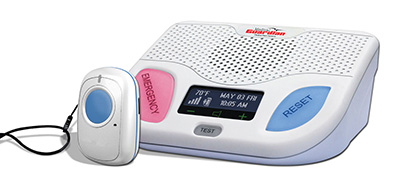
\includegraphics[scale=0.7]{medical-guardian-fall-alert-system}
	\caption{Medical Guardian Fall Alert System \cite{figure_guardian}}
\end{figure}
  
Another device on the market is myHalo$^{TM}$ from MobileHelp$^{TM}$. This device has more advantages compared to Medical Guadian one because of full body monitoring functions. It can detect a fall, mornitoring heart rate, skin temperature, sleep/wake pattern, etc. and send an alert signal to the authorized contacts. This product supports the medical alert outside the home powered by a nationwide cellular network and does not require landline phones. It also provides precise location of patients when they go outside with integrated mobile GPS system. This enable emergency call center to pinpoint patients' location and direct medical support to them. This service costs from \$41.95 per month and supports 24/7. However, because this system offers so many features, it seems to less focus on the fall detection. 

 \begin{figure}[h!]
	\centering
	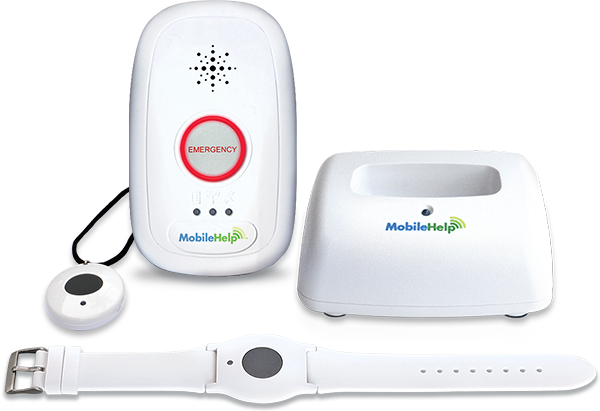
\includegraphics[scale=0.5]{mobile-help}
	\caption{myHalo Medical Alert System from MobileHelp$^{TM}$  \cite{myHalo}}
\end{figure}

\section{Existing Products from Other Research Groups}
Beside many commercial fall detection devices being available on the market, there are still many products from different research groups surrounding the fall detection topic. A group of Qiang Li and colleagues has used TEMPO (Technology-Enabled Medical Precision Observation) 3.0 sensor node for their project \cite{li}. This sensor node contains one tri-axial accelerometer and one tri-axial gyroscope and is controlled by an TI MSP430F1611 microcontroller. This group proposed an algorithm which combines the data from both accelerometer and gyroscope to reduce both false positive and false negative detection and improving the fall detection accuracy. This system is low in computational requirements and able to give a real-time response. The authors stated that their method has difficulties in differentiating jumping into bed and falling against a wall with a seated posture. 

 \begin{figure}[h!]
	\centering
	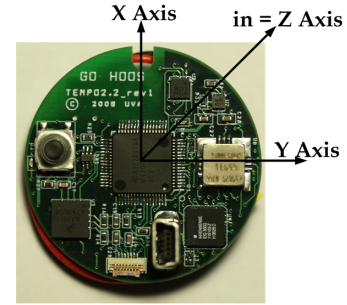
\includegraphics[scale=0.8]{tempo}
	\caption{TEMPO 3.0 sensor node \cite{li}}
\end{figure}

Binh Nguyen and Jonathan Tomkun designed and created a fall detection system for the elderly as a wearable monitoring device which can distinguish between fall and non-fall events  \cite{binh}. This device can link wirelessly with a pre-programmed laptop computer or Bluetooth-compatible mobile phone. Upon detecting a fall, the device communicates wirelessly with the laptop or cellphone to call 911 or issued emergency contacts. This device can also detect abnormal tilt and warns the user to correct their posture to minimize the risk of falling. In addition to visual LED to alert the fall, there are also audio and tacticle alert options for people with hearing or seeing disabilities. Regarding the performance of the system, some actions have not been distinguished by one of four proposed algorithms to be falls or non-falls. 

 \begin{figure}[h!]
	\centering
	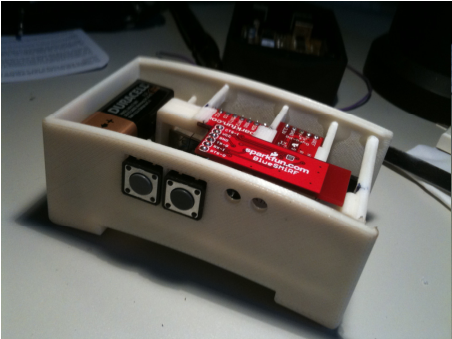
\includegraphics[scale=0.7]{binhnguyen_device}
	\caption{The final design of device from group research of Binh Nguyen and Jonathan Tomkun \cite{binh}}
\end{figure}  

\chapter{Statement of Problem and Methodology}

\section{Problem}
Nowadays, there have been various research groups studying on the area of fall detection on humans. The majority of them focus on designing a new algorithm to successfully distinguish between fall and fall-like activities. From the first time, most research groups used algorithms mainly based on the data from only one accelerometer such as \cite{only_accel_1},\cite{only_accel_2},\cite{only_accel_3}. However, focusing only on the data from the accelerometer can result in many false positives as other activities such as sitting, running and jumping may cause large peak accelerations. After that, there are other algorithms which rely on the detection of the body orientation after the fall such as \cite{body_orientation_1},\cite{body_orientation_2}. The main drawback of these strategies is that the fall can be confused by activities with similar postures such as sleeping, reclining, etc. It is also less effective when a person's fall posture is not horizontal. Then, there are some groups who have nominated such complex algorithms that used Support Vector Machine (SVM)\cite{SVM} and Markov model \cite{markov} to detect the fall. These techniques require a huge amount of computational resources which cause a delay which effects the robustness and accuracy of the system. 	
\section{Methodology and Algorithm}
From the disadvantages of prior works as mentioned above, this project proposes using an algorithm which combines data from one accelerometer and one gyroscope to detect the fall. The data from the accelerometer provides valuable information regarding body inertial change due to impact, while the gyroscope's data provides information about the body's rotational velocity during a fall event. This method helps improving the accuracy of the falling detection system without the need of complex computations.  \par
This algorithm is nominated by Quoc T. Huynh \textit{et al.} \cite{main_quoc}, which used data from both accelerometer and gyroscope sensors with predefined critical thresholds, to detect a fall with maximum sensitivity and specificity. Two parameters used to analyze in this algorithm are normalized acceleration and normalized angular velocity. \par

Normalized acceleration is the total sum acceleration vector, named $\boldsymbol{Acc_{norm}}$, containing both static and dynamic acceleration components in different directions. This parameter is calculated with the formula below 

\begin{equation}
\boldsymbol{Acc_{norm}}=\sqrt{(A_x)^2+(A_y)^2+(A_z)^2}
\end{equation}
where $A_x$, $A_y$ and $A_z$ represent the acceleration of three directions $\textit{x, y, z}$. \par 
Normalized angular velocity is the total sum angular velocity vector, named $\boldsymbol{\omega_{norm}}$, containing the rotational velocity components in different directions. This parameter is calculated with the formula below

\begin{equation}
\boldsymbol{\omega_{norm}}=\sqrt{(\omega_{x})^2+(\omega_{y})^2+(\omega_{z})^2}
\end{equation}
where $\omega_x$, $\omega_y$ and $\omega_z$ represent the angular velocity of three directions \textit{x, y, z}.

When it stays in stationary condition, the body of the user gives the acceleration magnitude of a constant at +1g and angular velocity at $0^{o}/s$. When the user falls, there is a rapid change in the body's acceleration while the angular velocity produces a variety of signals in the fall direction. To detect the fall, the acceleration and angular velocity are compared with critical thresholds. These thresholds are defined as followed by Quoc T. Huynh \textit{et al.} \par 
{\addtolength{\leftskip}{1.5cm}
(a) \textit{Lower fall threshold(LFT)}: local minima for the Acc
resultant of each recorded activity are referred to
as the signal lower peak values (LPVs). The $LFT_{Acc}$
for the acceleration signals is set at the level of the
smallest magnitude lower fall peak (LFP) recorded.\par
}
{\addtolength{\leftskip}{1.5cm}
	(b) \textit{Upper Fall Threshold(UFT)}: local maxima for the Acc and $\omega$
	resultant of each recorded activity are referred to as
	the signal upper peak values ($UPV_{s}$). The UFT for
	each of the acceleration ($UFT_{Acc}$) and the angular
	velocity ($UFT_{Gyro}$) signals are set at the level of the
	lowest upper fall peak (UFP) recorded for the $\boldsymbol{Acc}$
	and $\boldsymbol{\omega}$, respectively. The $UFT_{Acc}$ is related to the peak
	impact force experienced by the body segment during
	the impact phase of the fall.\par
}
\cleardoublepage
When a fall happens, the normalized acceleration first falls below the $LFT_{Acc}$ threshold
which indicates the start of a fall event. In the next 0.5 seconds, usually called fall windows,
data from both accelerometer and gyroscope are compared to $UFT_{Acc}$ and $UFT_{Gyro}$. The fall windows was obtained from the literature \cite{window_1}\cite{window_2}. If
the magnitude of both parameters exceed the two upper thresholds, a fall is detected.
However, if only one of these conditions is not satisfied, there is no fall detection. Quoc T.
Huynh et al. \cite{main_quoc} have proven, with practical experiments on real subjects, that the three
conditions above just happen simultaneously only with a fall but not other activities like
standing, running, jumping of sitting up. Figure 3.1 summarizes the main steps of this
algorithm.
\cleardoublepage
\begin{figure*}
	\centering
	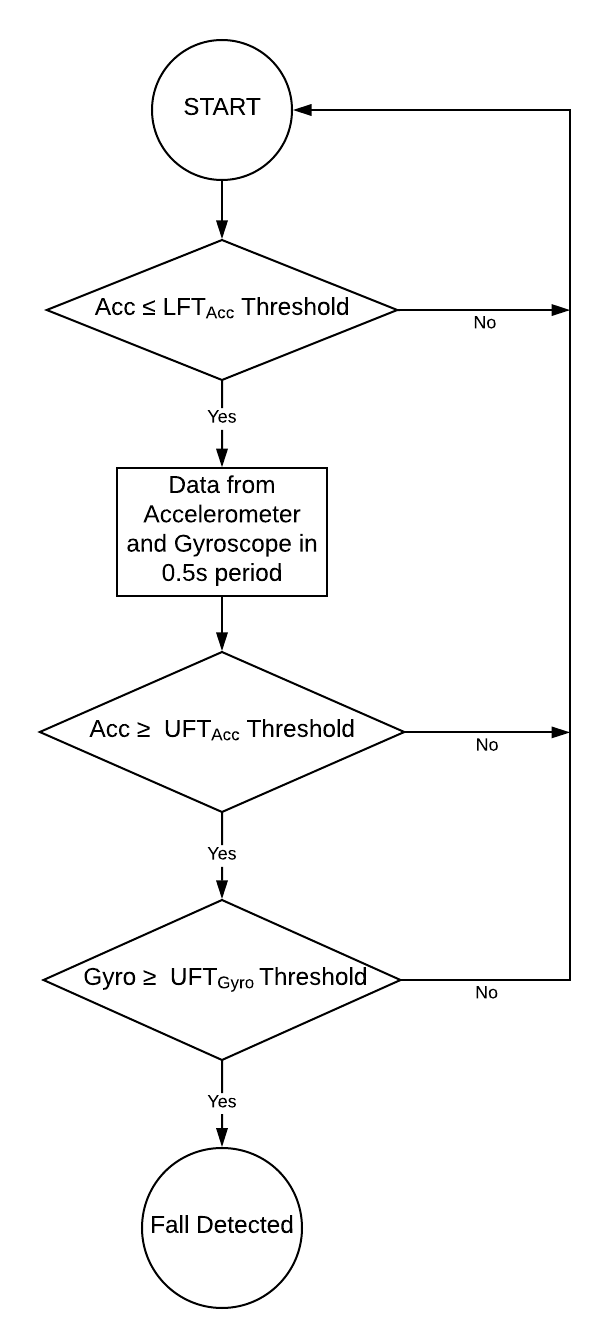
\includegraphics[scale=0.8]{algorithm_diagram}
	\caption{Fall detection algorithm}
\end{figure*}
\cleardoublepage

\chapter{System overview}

\section{Hardware Components}

\subsection{Sensor}
Since the algorithm requires information of both acceleration and angular velocity, an \gls{imu} named MPU6050 from Invensense\textregistered, which contains one accelerometer and one gyroscope, has been chosen for its convenience. This sensor can also accepts inputs from an external 3-axis compass via I$^{2}$C sensor bus to provide a complete 9-axis MotionFusion$^{TM}$ output.
 \begin{figure}[h]
	\centering
	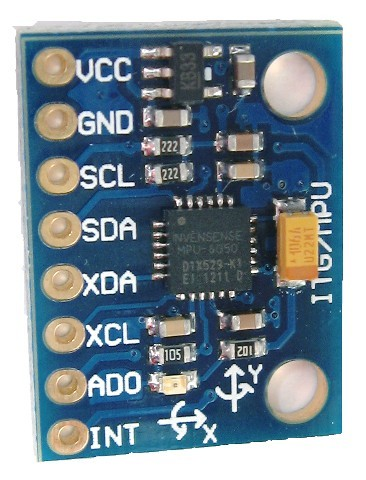
\includegraphics[scale=0.25]{mpu6050}
	\caption{MPU-6050 by Invensense \cite{mpu}}
\end{figure}\\
The accelerometer inside the MPU6050 board can measure the acceleration in four different programmable full-scale ranges ($\pm2g$, $\pm4g$, $\pm8g$ and $\pm16g$). An integrated 16-bit \gls{adc} supports simultaneous sampling of the accelerometer while requiring no external multiplexer. This accelerometer normally operates at a very small current of \SI{500}{\micro\ampere} with low power consumption. 
According to the data-sheet given by Invensense\textregistered, the raw output of the accelerometer is displayed in form of LSB/g. Divided with an appropriate \gls{ssf}, we can obtain the acceleration in g - standard gravity unit, which is used in this project. Each full scale has its own SFF. Table 4.1 shows different full-scales of the accelerometer and table 4.2 shows the \gls{ssf} for each scale.
\cleardoublepage
\begin{table}[h!]
	\begin{center}
		\begin{tabular}{ |c|c|c|c| } 
			\hline
			Scale & TYP & UNIT \\
			\hline
			\verb|AFS_SEL=0| & $\pm2$ & g \\ 
			\verb|AFS_SEL=1|& $\pm4$ & g \\ 
			\verb|AFS_SEL=2|& $\pm8$ & g \\
			\verb|AFS_SEL=3|& $\pm16$ & g\\
			\hline
		\end{tabular}
		\caption{Full-scale Range Table of Accelerometer}
		\label{table:1}
	\end{center}
\end{table}
\begin{table}[h!]
	\begin{center}
		\begin{tabular}{ |c|c|c|c| } 
			\hline
			Scale & Sensitivity Scale Factor & UNIT \\
			\hline
			\verb|AFS_SEL=0| & 16,384 & LSB/g \\ 
			\verb|AFS_SEL=1|& 8,192 & LSB/g \\ 
			\verb|AFS_SEL=2|& 4,096 & LSB/g \\
			\verb|AFS_SEL=3|& 2,048 & LSB/g\\
			\hline
		\end{tabular}
		\caption{Sensitivity Scale Factor Table of Accelerometer}
		\label{table:1}
	\end{center}
\end{table}
With \verb|AFS_SEL| being bits of the accelerometer configuration register of the sensor. These bits are used to select the full scale range of the accelerometer. \par 

 The gyroscope integrated on the same board can measure the angular velocity at 4 programmable full-scale ranges ($\pm250^{o}/s$, $\pm500^{o}/s$, $\pm1000^{o}/s$ and $\pm2000^{o}/s$). This sensor has an external sync signal which supports image, video capturing and GPS synchronization. Its normal operating current is \SI{500}{\micro\ampere} which enables the reduction on power consumption. The raw output of the gyroscope is displayed in form of LSB/($^{o}/s$). Divided with an appropriate Sensitivity Scale Factor (\gls{ssf}), we can obtain the angular velocity with unit of ($^{o}/s$). Each full scale has its own SFF. Table 4.3 shows different full-scale of the gyroscope and table 4.4 shows the \gls{ssf} for each scale. 
\begin{table}[h!]
	\begin{center}
		\begin{tabular}{ |c|c|c|c| } 
			\hline
			Scale & TYP & UNIT \\
			\hline
			\verb|FS_SEL=0| & $\pm250$ & $^{o}/s$\\ 
			\verb|FS_SEL=1|& $\pm500$ & $^{o}/s$ \\ 
			\verb|FS_SEL=2|& $\pm1000$ & $^{o}/s$ \\
			\verb|FS_SEL=3|& $\pm2000$ & $^{o}/s$\\
			\hline
		\end{tabular}
		\caption{Full-scale Range Table of Gyroscope}
		\label{table:1}
	\end{center}
\end{table}
\begin{table}[h!]
	\begin{center}
		\begin{tabular}{ |c|c|c|c| } 
			\hline
			Scale & Sensitivity Scale Factor & UNIT \\
			\hline
			\verb|FS_SEL=0| & 131 & LSB/($^{o}/s$) \\ 
			\verb|FS_SEL=1|& 65.5 & LSB/($^{o}/s$) \\ 
			\verb|FS_SEL=2|& 32.8 & LSB/($^{o}/s$) \\
			\verb|FS_SEL=3|& 16.4 & LSB/($^{o}/s$)\\
			\hline
		\end{tabular}
		\caption{Sensitivity Scale Factor Table of Gyroscope}
		\label{table:1}
	\end{center}
\end{table}
\newpage
With \verb|FS_SEL| being bits of the gyroscope configuration register on the sensor. These bits are used to select the full scale range of gyroscope. \par 
After getting acceleration and angular velocity in three different directions from two sensors, normalized acceleration and normalized angular velocity are calculated with formulas (3.1) and (3.2) and compared with thresholds to detect the fall. 
\subsection{Microcontroller}
To perform all data processing and communications, the ESP8266EX \gls{mcu} integrated with L106 32-bit RISC processor from Tensilica is chosen. This \gls{mcu} archives extra low power consumption and reaches a maximum clock speed up to 160 MHz, which is specially designed for mobile and \gls{iot} applications. The ESP8266EX \gls{mcu} supports most of popular interfaces such as GPIO, UART, I$^{2}$C, ADC, PWM etc. to connect with external peripheral devices. Figure 4.3 shows the functional block diagram of ESP8266EX. \par 
\begin{figure}[h]
	\centering
	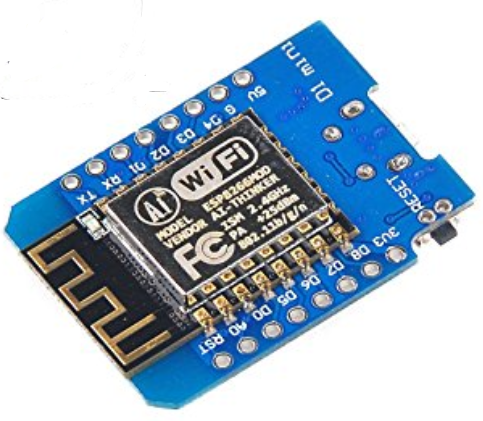
\includegraphics[scale=0.5]{esp8266}
	\caption{ESP8266 D1 Mini Board with an ESP8266EX MCU inside}
\end{figure}
\cleardoublepage
\begin{figure}[h]
	\centering
	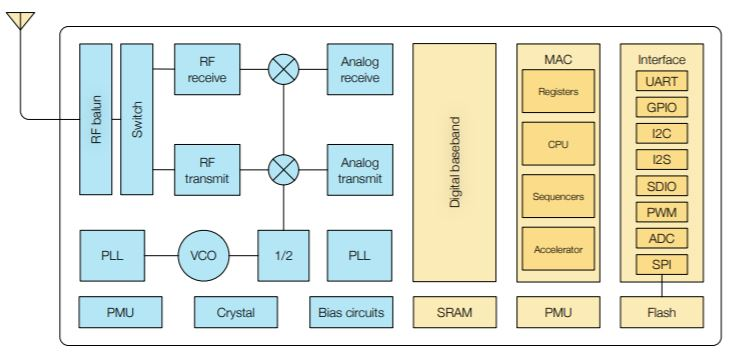
\includegraphics[scale=0.8]{functional_diagram}
	\caption{Functional Block Diagram of ESP8266EX MCU\cite{block_diagram}}
\end{figure}
The ESP8266EX \gls{mcu} integrates memory units including one 50kB SRAM and one 16MB external SPI flash that are sufficient for most \gls{iot} applications. The SRAM size is less than 50kB when the \gls{mcu} is working under Station Mode or connecting to a router. All user programs are stored in the external SPI flash and non-volatile after switching off the power.
\subsection{Wireless Module}
ESP8266EX \gls{mcu} integrates a Wi-Fi module in which is implemented TCP/IP protocol with the full 802.11 b/g/n WLAN MAC standard and Wi-Fi Direct specification. The ESP8266EX is designed with advance power management technologies. The low-power architecture operates in three modes: active mode, sleep mode and deep-sleep mode. ESP8266 consumes only\SI{20}{\micro\ampere} in deep-sleep mode and the standby power consumption below 1.0mW. These two features make the ESP8266 Wi-Fi module fully compatible with mobile wireless applications that require low power dissipation. \par
In this project, a standard TCP/IP protocol has been chosen because of its highly reliable connection and its ability to control data congestion. Additionally, this system also requires that the received data on the monitoring computer must be in the same order as the original one on the sensor module. Therefore, TCP/IP is chosen because of its capability of ordering the received data and error recovery. Whenever there is an error on the connection, all the erroneous packets are retransmitted to the destination and rearranged in the correct order.\par 
A brief description of the wireless communication system: there is a TCP server running on the monitoring computer and listening to the requests from the clients. The ESP8266 module (programmed in \textit{client mode}) continuously sends sensors' data to the server via a Wi-Fi connection. All data is captured by a Python program and plotted on a visual graph. The received data is also stored in a database to serve later data analysis and algorithm optimization. 
\begin{figure}[h!]
	\centering
	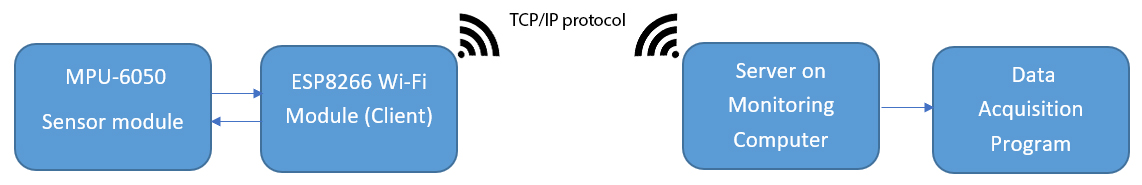
\includegraphics[scale=0.38]{system_schematic}
	\caption{Schematic of wireless communication system}
\end{figure} 
\section{Software}

\subsection{Embeddded Software on the Sensor Node}
On the sensor node, the micro-controller board is programmed to read the data from sensors, calculate normalized parameters and send data to the host computer. First, the microcontroller communicates with sensors, using I$^{2}$C protocol with the help of MPU6050 library written by Jeff Rowberg \cite{mpu_lib}, to set clock source and full scale range for two sensors. It is also important to set the sensor board to wake-up mode in this step to make sure it is working.  After successfully connecting, the frequency of these two sensors are set to 1kHz by configuring the digital low pass filter with the \textit{setDLPFMode} function from the library. Normally, these sensors operate at the frequency of 8kHz, which means there are 8000 output samples within one second. That is too much compared to the requirement of a fall detection system and usually causes congestion and lost data during the transmission from the sensor node to the host computer. To avoid this problem, it is necessary to slow down the internal sampling rate of the two sensors. See the table 4.5 for the digital low pass filter configuration. \clearpage
\begin{table}[h!]
	\begin{center}
		\begin{tabular}{ |c|c|c|c|c|c| } 
			\hline
			 & \multicolumn{2}{c|}{Accelerometer} & \multicolumn{2}{c|}{Gyroscope} &  \\
			 \cline{2-5}
			 \verb|DLPF_CFG| & Bandwidth & Delay & Bandwidth & Delay & Sample Rate\\ 
			 \hline
			 0 & 260Hz & 0ms & 256Hz & 0.98ms &8kHz \\
			 \hline
			 1 & 184Hz & 2.0ms & 188Hz & 1.9ms & 1kHz\\
			 \hline
			 2 & 94Hz & 3.0ms & 98Hz & 2.8ms & 1kHz\\
			 \hline
			 3 & 44Hz & 4.9ms & 42Hz & 4.8ms & 1kHz\\
			 \hline
			 4 & 21Hz & 8.5ms & 20Hz & 8.3ms & 1kHz\\
			 \hline
			 5 & 10Hz & 13.8ms & 10Hz & 13.4ms & 1kHz\\
			 \hline
			 6 & 5Hz & 19.0ms & 5Hz & 18.6ms & 1kHz\\
			 \hline
		\end{tabular}
		\caption{Digital Low Pass Filter Configuration of the MPU-6050 Sensor}
	\end{center}
\end{table}
Next, like other sensors, both gyroscope and accelerometer always have non-zero errors even when leveling and need to be calibrated with a set of offset values before being used. These offsets are calculated by another program included in the MPU6050 library and set into appropriate sensor's registers with the provided function from the library. See the appendix C for the register map of the MPU6050 sensor. \par
After initializing the sensors, the sensor node establishes a wireless connection with the local network and host computer. While the host computer is not connected, the sensor node continuously calls for a connection and the LED indicator on the micro-controller board keeps brighting until receiving a successful connection. Once the connection is established, the sensor node turns off the indicator LED for a while and then starts blinking while transferring data. All the connection handling functions are included in the \textit{Connection Handling} library written by myself. See the Appendix B.\par 

Finally, the micro-controller starts reading data from the two sensors with the function \textit{getMotion6}. The output data is used to calculate the normalized acceleration and angular velocity. Whenever the normalized acceleration falls below the $LFT_{Acc}$ threshold, the first flag is set true to indicate the start of a fall event and a 500ms timer starts counting. For the next 500ms, if normalized acceleration and angular velocity exceed the $UFT_{Acc}$ and $UFT_{Gyro}$ respectively, the second and third flags are also set true. When the timer is executed, all flags are checked. If three flags are all true, a fall is detected. The sensor node will send an emergency email to the caregivers while it starts blinking the super bright red led simultaneously. That red led helps the caregivers to find the patient when they reach the patients' location. If one condition is not true, the system would reset all flags and start a new detection loop. All the reading data are also converted into strings, concatenated in comma-separated form and sent to the host computer for monitoring. Each message is ended with a new line character to separate them on the PC side. See Appendix A for the main code on the sensor node. 
\subsection{Data Acquisition Software}
Data acquisition software is written in Python programming language with Pycharm environment because of its convenience and full support. This software starts an always-run server on the host computer and waits for the requests from the client. When receiving a message from the client, the software de-concatenates this message into two arrays which contain acceleration and angular velocity values separately.  Data from two arrays are then converted back to float form and visualized on the graph. These values are also written to text files in comma-separated (.CSV) form and stored for future analysis with MATLAB. Figure 4.5 shows the graphic user interface of this software. See the Appendix D for the code. 
 
\begin{figure}[h!]
	\centering
	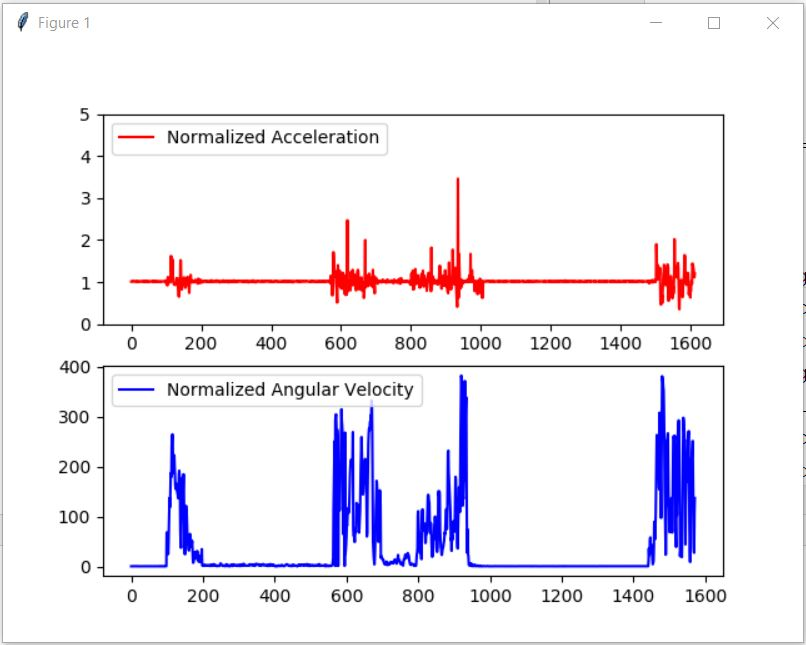
\includegraphics[scale=0.7]{data_program}
	\caption{Graphic User Interface of Data Acquisition Program}
\end{figure} 
\subsection{Data Analysis Software}
MATLAB is used to analyze the collected data from the experiments. Data stored in the CSV file is first loaded to MATLAB arrays with MATLAB function \textit{csvread}. Data after being loaded to arrays is visualized with the plotting function supported by MATLAB. While working with the data, we can use the data cursor tool provided by MATLAB to figure out the valued of upper and lower peaks (Figure 4.6).
\begin{figure}[h!]
	\centering
	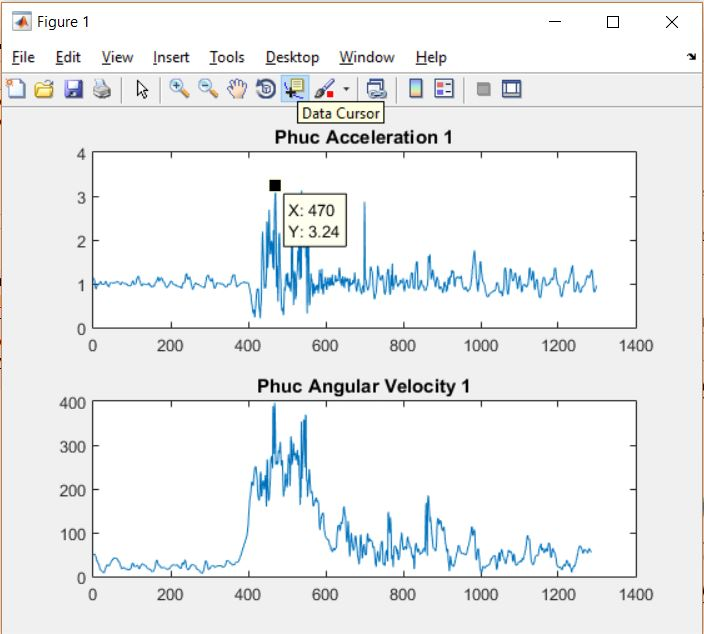
\includegraphics[scale=0.7]{matlab_window}
	\caption{Data plotting with MATLAB}
\end{figure}
\section{System Intergration}
The communication between micro-controller and sensor board is established with I$^{2}$C interface. 	This interface uses only two wires named SCL(serial clock) and SDA(serial data) and both of them need to be pulled up with resistors to +Vdd. I$^{2}$C interface is popular to use because of its ability to support low-speed device such as micro-controller, EEPROM, I/O interface or A/D and D/A converters.  
\cleardoublepage
\begin{figure}[h]
	\centering
	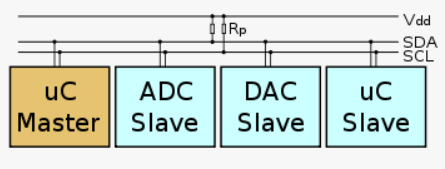
\includegraphics{I2C}
	\caption{Principle of I$^{2}$C interface \cite{i2c}}
\end{figure}\par
I$^{2}$C transfers every 8 bits (byte) and uses 7-bit address to communicate with a certain device. Bit 0 is set to 0 or 1 to define the signal reading from or writing to the device. Every device has its own unique address and multiple devices (slaves) can connect to a single \gls{mcu} (master) on only one I$^{2}$C bus. With this feature, both the accelerometer and gyroscope can connect to the ESP8266EX \gls{mcu} with only one bus. Figure 3.3 shows the connection between MPU6050 \gls{imu} and ESP8266 board.
\begin{figure}[h!]
	\centering
	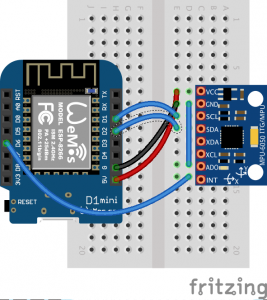
\includegraphics[scale=0.6]{mpu6050-esp8266}
	\caption{Wiring schematic of MPU-6050 \gls{imu} \cite{d1sche}}
\end{figure} \par
To suffice the compact and portable requirement of the sensor node, sensor board and micro-controller are connected together on the Printed Circuit Board (PCB) with the dimension of 60x40mm (Figure 4.9). All the sensor node is powered by a power-shield especially designed for the ESP8266 D1 Mini Board. This shield supports the Lithium-Ion Polymer battery with JST-PH connector and allows the user to re-charge the battery with a USB cable. It is convenient for the user to charge the device everyday with the micro-USB cable which can be found everywhere. Figure 4.8 is the final design of the sensor node.
\cleardoublepage
\begin{figure}[h!]
	\centering
	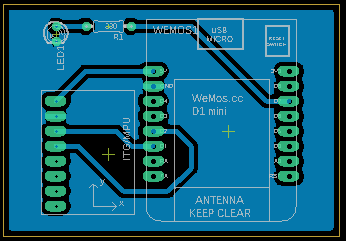
\includegraphics[scale=2]{pcb_design}
	\caption{Printed Circuit Board Design}
\end{figure}
\vspace{2cm}
\begin{figure}[h!]
	\centering
	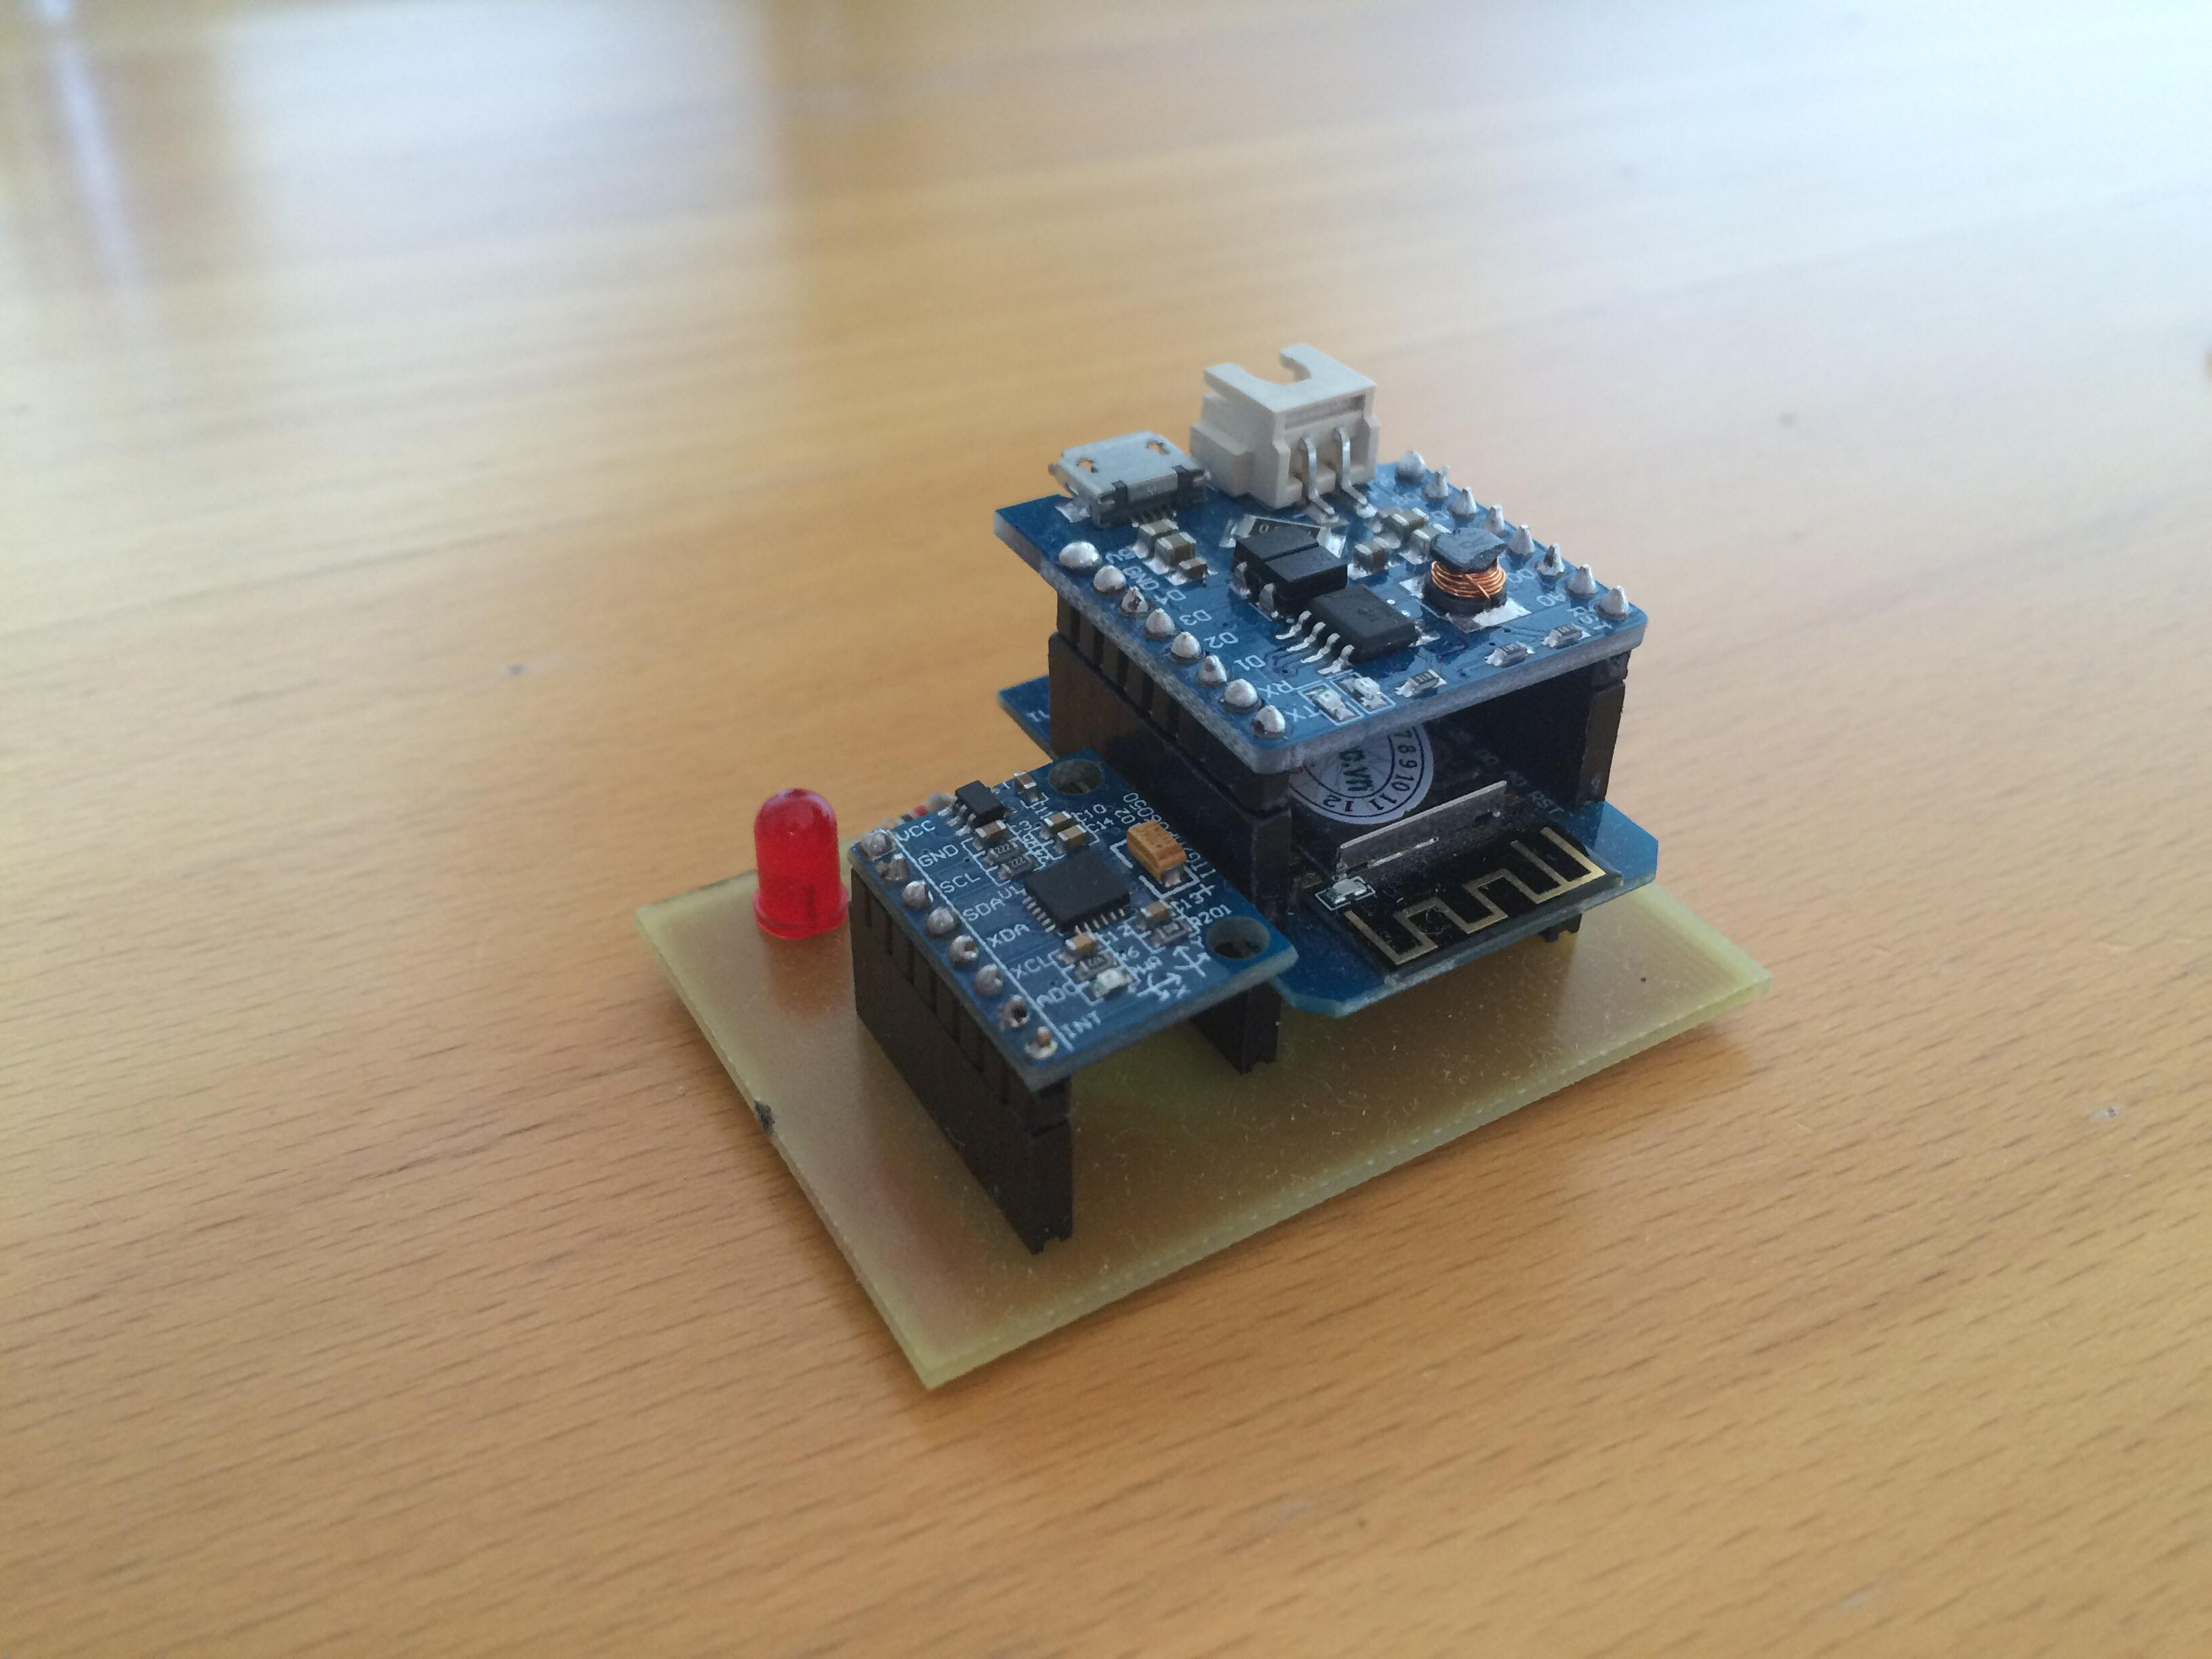
\includegraphics[scale=0.13]{final_product}
	\caption{Sensor Node}
\end{figure}
\chapter{Experimental and Procedure}

\section{Data Collection Method}
To collect the data of falls and fall-liked activities for the development and optimization of the falls detection algorithm, experiments were performed on 5 young healthy subjects (male volunteers, age of 22 years old, weight from 60 to 90kg and height from 160 to 180 cm) to simulate the \gls{adl} and falls. These subjects are numbered from S1 to S6 with detail information provided below.
\begin{table}[h]
	\begin{center}
		\begin{tabular}{ |c|c|c|c|c| } 
			\hline
			Subject & Age(years) & Height & Weight(Kg) & Gender \\
			\hline
			S1 & 22 & 167 & 55 & M\\ %hieu
			S2 & 22 & 179 & 71 & M\\ %huy
			S3 & 22 & 170 & 90 & M\\ %minh
			S4 & 22 & 178 & 65 & M\\ %phuc
			S5 & 22 & 170 & 90 & M\\ %trung	
			\hline
		\end{tabular}
		\caption{Detail body information of volunteers}
		\label{table:1}
	\end{center}
\end{table}\par
All the subjects were asked to perform different movements such as standing, sit down/stand up, step, run, lying on the bed, go up/down the stair and different fall test including forward, backward, right/left side way. The sensor node is attached to the center of chest, where was determined to be the optimal place for sensor placement. To ensure the safety of volunteers, all the experiments were conducted on a 36-cm high cushion at the dormitory.
\section{Data Analysis}
Figure 5.1 is the visualized data of two typical fall events collected on volunteers S1 and S4. From two data set in the figure, it is clear that when a fall happen, the normalized acceleration first falls to a certain point below the normal acceleration to indicate the start of a fall. Within the next 0.5s, the normalized acceleration from two experiments both rise up to the upper peak at around 2.8 - 3.2 g and then return to the normal level. During the fall, the normalized angular velocity of both experiments also reach the peaks at around 327 - 396$^{o}/s$. This patterns can be met in most of other fall experiments with other volunteers (see appendix E) and agree with the pattern that was stated by the algorithm in section 3.2. It is a confirmation for the accuracy of the theory founded by Huynh \textit{et al.} \cite{main_quoc}.\\

\begin{figure}[h!]
	\centering
	\hspace{-2.5cm}
	\begin{minipage}[b]{0.5\textwidth}
		\centering
		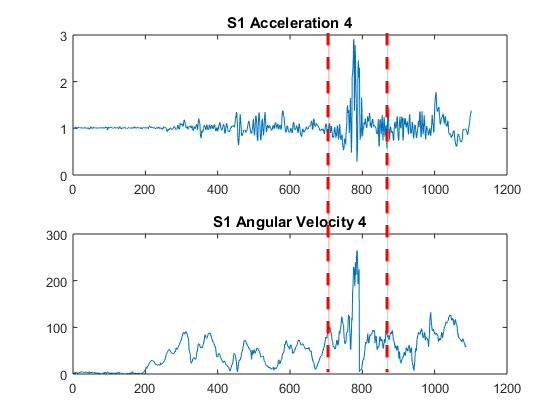
\includegraphics[scale=0.5]{hieu4}
		(a) S1 falls forward
	\end{minipage}%
	\hfill
	\begin{minipage}[b]{0.5\textwidth}
		\centering
		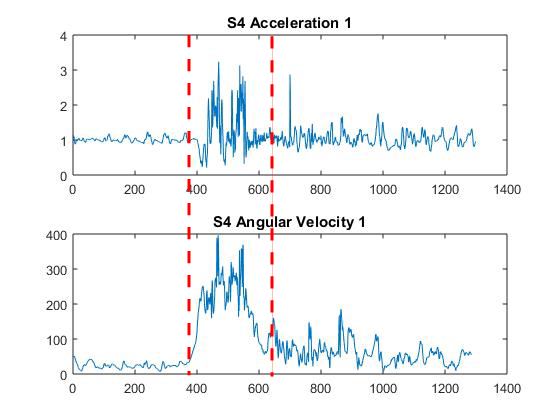
\includegraphics[scale=0.5]{phuc1}
		(b) S4 falls right sideway
	\end{minipage}	
	\caption{Fall forward data}
\end{figure}
The collected data of falls on five volunteers are represented in the table 5.2. This table demonstrates the comparison between the peak values resulted by different subjects when they performed different fall simulations. This table help me to determine three thresholds by using observation method.\par  
First, it is important to find the optimal Lower Fall Threshold for the acceleration ($LFT_{Acc}$), because it is the first condition to start detecting a fall. Improper selection of the $LFT_{Acc}$ may lead to the miss of the fall event and cause failure of fall detection. From the given data in table, most of the lower peaks are below 0.35 g. To ensure the system can detect most of the fall, I decided to choose the Lower Fall Threshold for the acceleration at 0.35g.
\par
For the upper peaks of the acceleration in all kind of falls, the value is in the range of 2.31 - 3.46 g. This data helped me choose the Upper Fall Threshold for the acceleration ($UFT_{Acc}$) at about 2.75, to make sure the acceleration during 90\% of all falls will exceed the upper threshold and satisfy the second condition of the fall detection algorithm. 
\par 
The final step is choosing the upper fall threshold for the angular velocity as a confirmatory threshold for the fall detection algorithm. From the data in table 5.2, it is suitable to choose the $UFT_{Gyro}$ at around 254$^{o}/s$.
\begin{table}[h]
	\begin{center}
		\begin{tabular}{ |c|c|c|c|c| } 
			\hline
			Subject & experiment & Lower Peak Acc (g) & Upper Peak Acc (g)  & Upper Peak Gyro ($^{o}/s$)\\
			\hline
			S1 & 1 & 0.23 & 3.24 & 282.9\\%hieu
			& 2 & 0.26 & 2.87 & 278.9 \\
			& 3 & 0.23 & 2.84 & 262.1 \\
			& 4 & 0.53 &  2.91 & 264.9 \\
			& 5 & 0.24 &  2.99 & 327.5\\
			\hline
			S2 & 1 & 0.22 & 2.77 & 350.9\\
			& 2 &  0.28 &  3.23 & 321.5\\
			& 3 &  0.08 &  2.83& 328.1\\
			& 4 & 0.13 & 2.74 & 314.3\\
			& 5 & 0.16 & 3.46 & 319.1\\  %huy
			\hline
			S3 & 1 & 0.33 &  3.22& 260.7 \\
			& 2 &  0.39 & 3.10 & 271.7 \\
			& 3 & 0.14 & 3.07 & 278.7\\
			& 4 & 0.03 & 2.31 & 327.1\\
			& 5 & 0.05 & 3.19 & 294.0\\ %minh
			\hline
			S4 &1 & 0.21 & 3.24 & 396.4\\ 
			&2 &  0.09 & 2.93 & 345.4\\ 
			&3 & 0.05 & 3.36 & 307.6\\ 
			&4 & 0.03 & 3.11 & 356.9\\ 
			&5 & 0.31 & 3.35 & 348.1\\ %phuc
			\hline
			S5 &1 & 0.14 & 3.46 & 433.3\\ 
			&2 &  0.07 & 3.35 & 385.3\\ 
			&3 & 0.08 & 2.96 & 362.9\\ 
			&4 & 0.12 & 3.21 & 343.8\\ 
			&5 & 0.31 & 3.28 & 278.1\\ %trung
			\hline
		\end{tabular}
		\caption{Collected data of simulated falls in different directions}
		\label{table:1}
	\end{center}
\end{table}
\cleardoublepage

\chapter{Results and Discussion}

\section{Results Assessment}

\section{Comparing the performance with existing works}

\chapter{Conclusion and Future Works}

\section{Summary}

\section{Limitations}

\section{Future works}
%======================================================================


\appendix
% Add a title page before the appendices and a line in the Table of Contents
\addcontentsline{toc}{chapter}{APPENDICES}
%======================================================================
\chapter{C/C++ Code on the Sensor Node}
\begin{lstlisting}
	#include <Event.h>
	#include <Timer.h>
	#include <AsyncPrinter.h>
	#include <async_config.h>
	#include <ESPAsyncTCP.h>
	#include <ESPAsyncTCPbuffer.h>
	#include "MPU6050.h"
	#include "Wire.h"
	#include "WiFiClient.h"
	#include "ESP8266WiFiMulti.h"
	#include "ESP.h"
	#include "Time.h"
	#include <CSensorSender.h>
	
	
	ESP8266WiFiMulti WiFiMulti ;
	#if I2CDEV_IMPLEMENTATION == I2CDEV_ARDUINO_WIRE
	#include "Wire.h"
	#endif
	#define OUTPUT_READABLE_ACCELGYRO
	//#define SERIAL_DEBUG
	#define BUZZER 13
	#define CONN_INTERVAL     (1000)
	#define NUMB_ELEMS_PACKET (100)
	#define SAMPL_INTV        (CONN_INTERVAL/NUMB_ELEMS_PACKET)
	#define dataRate 9
	#define lowAcc 0.26
	#define highAcc 2.75
	#define highGyro 254.5
	
	Timer t;
	const uint16_t port = 8000;
	String host = "192.168.137.1"; // ip or dns
	
	CSensorSender mySender(host, port, NUMB_ELEMS_PACKET, 2);
	
	// Use WiFiClient class to create TCP connections
	AsyncClient client;   
	MPU6050 accelgyro;
	
	//MPU6050 accelgyro(0x69); // <-- use for AD0 high
	int16_t ax, ay, az;
	int16_t gx, gy, gz;
	float t_time = 0,send_time;
	float rotX, rotY, rotZ,normAcc;
	float gyroX, gyroY, gyroZ, normGyro;
	String packet = "",packetSend = "";
	int8_t i=0;
	bool blinkState = false;
	bool firstCond = false, secCond = false, thirdCond = false;
	
	void Print_IMU()
	{
			#ifdef SERIAL_DEBUG
			Serial.println("Accelerometer:");
			Serial.print(ax);
			Serial.print("\t");
			Serial.print(ay);
			Serial.print("\t");
			Serial.println(az);
			Serial.println("Gyroscope: ");
			Serial.print(gx);
			Serial.print("\t");
			Serial.print(gy);
			Serial.print("\t");
			Serial.println(gz);
			#endif
			Serial.print(normAcc);
			Serial.print(" ");
			Serial.println(normGyro);
	}
	void alert(){
			if (firstCond == true && secCond == true && thirdCond == true)
			{
				digitalWrite(BUZZER, HIGH);
			}
			firstCond = false;
			secCond = false;
			thirdCond = false;
	}
	void init_IMU() {
			// join I2C bus (I2Cdev library doesn't do this automatically)
			Wire.begin();
			Serial.begin(115200);
			// initialize device
			Serial.println("Initializing I2C devices...");
			accelgyro.initialize();
			// verify connection
			Serial.println("Testing device connections...");
			Serial.println(accelgyro.testConnection() ? "MPU6050 connection successful" : "MPU6050 connection failed");
			Serial.print("\n");
			accelgyro.setDLPFMode(1); //set the Frequency to 1kHz
			accelgyro.setRate(dataRate); //Set data Rate: Rate = (Freq)/(dataRate+1)
			Serial.print("DLPF Mode: ");
			Serial.println(accelgyro.getDLPFMode());
			Serial.print("Data rate of sensor: ");
			Serial.println(accelgyro.getRate());
			// use the code below to change accel/gyro offset values
			Serial.println("Updating internal sensor offsets...");
			accelgyro.setXGyroOffset(55);
			accelgyro.setYGyroOffset(-28);
			accelgyro.setZGyroOffset(-2);
			accelgyro.setXAccelOffset(-2581);
			accelgyro.setYAccelOffset(-3937);
			accelgyro.setZAccelOffset(1199);
	}
	void Init_Wifi()
	{
			// Initialize Wifi_connection
			WiFiMulti.addAP("MinhKhang", "qwertyuiop");
			Serial.println();
			Serial.println();
			Serial.print("Wait for WiFi... ");
			while(WiFiMulti.run() != WL_CONNECTED) {
			Serial.print(".");
			delay(500);
			ESP.wdtFeed();
			}
			Serial.println("");
			Serial.println("WiFi connected");
			Serial.println("IP address: ");
			Serial.println(WiFi.localIP());
			digitalWrite(2, LOW);
			delay(500);
	}
	
	void setup(){
			//initialize pin mode
			pinMode(BUZZER, OUTPUT);
			Serial.begin(115200);
			Wire.begin();
			init_IMU();
			Init_Wifi();
	}
	void loop() {
			sensorData_t;
			ESP.wdtFeed();
			if ((millis()-t_time)>SAMPL_INTV)
			{ 
				//get data from sensor
				accelgyro.getMotion6(&ax, &ay, &az, &gx, &gy, &gz);
				rotX = ax / 16384.0;
				rotY = ay / 16384.0;
				rotZ = az /16384.0;
				normAcc = sqrt(rotX*rotX + rotY*rotY + rotZ*rotZ);
				gyroX = gx /131.0;
				gyroY = gy /131.0;
				gyroZ = gz /131.0;
				normGyro = sqrt(gyroX*gyroX + gyroY*gyroY + gyroZ*gyroZ);
				//Start the comparator
				if (normAcc < lowAcc)
				{
					firstCond = true;
					t.after(500,alert);
				}
				if (firstCond == true && normAcc > highAcc)
				{
					secCond = true;
				}
				if (firstCond == true && normGyro > highGyro)
				{
					thirdCond =true;
				}
				t_time=millis();
				currentSensorData.normAccel = normAcc;
				currentSensorData.normGyro = normGyro;
				mySender.queueSensorData(currentSensorData);
			}
			t.update();
	}
\end{lstlisting}%

\chapter{Connection Handling Library}

\begin{lstlisting}
	#include "CSensorSender.h"
	
	#define DEBUG_PRINT 1
	
	static inline void debugPrint(String inputString)
	{
		#if DEBUG_PRINT
		Serial.println(inputString);
		#endif
	}
	
	void clientConnectedHandler(void* arg, AsyncClient* aClient)
	{
		debugPrint("Connected");
		String sentString = ((CSensorSender*)arg)->getSentString();
		aClient->write(sentString.c_str());
		((CSensorSender*)arg)->setIndicatorLed(LOW);
	}
	
	void clientDisconnectedHandler(void* arg, AsyncClient* aClient)
	{
		debugPrint("Disconnected");
		senderState_t senderState = ((CSensorSender*)arg)->getSenderState();
		if ((senderState == SENDING) || (senderState == SENDING_ERROR)) {
			((CSensorSender*)arg)->setSenderState(READY);
		}
		((CSensorSender*)arg)->setIndicatorLed(HIGH);
	}
	
	void clientErrorHandler(void* arg, AsyncClient* aClient, unsigned char error)
	{
		debugPrint("Error");
		senderState_t senderState = ((CSensorSender*)arg)->getSenderState();
		if (senderState == SENDING) {
		((CSensorSender*)arg)->setSenderState(SENDING_ERROR);
		}
		((CSensorSender*)arg)->setIndicatorLed(HIGH);
	}
	
	void CSensorSender::populateSentString()
	{
		mSentString = "";
		for (int i = 0; i < mNoOfSamples; i++) {
		mSentString += String(mSensorData[i].normAccel) + "," + String(mSensorData[i].normGyro);
			if (i < mNoOfSamples - 1) {
				mSentString += ",";
			}
			else {
				mSentString += "\n";
			}
		}
	}
	
	// Constructor
	CSensorSender::CSensorSender(String IPString, int16_t port, uint16_t noOfSamplesPerPacket, int ledIndicatorPin)
	{
		// Load the arguments onto the attributes
		mIPString = IPString;
		mPort = port;
		mNoOfSamplesPerPacket = noOfSamplesPerPacket;
		// Allocate the exact number of elements of sensorData_t
		// this is going to be the array to store queued data
		mSensorData = new sensorData_t[mNoOfSamplesPerPacket];
		mSentString = "";
		mNoOfSamples = 0;
		// Initialize the state to READY
		mSenderState = READY;
		mLedIndicatorPin = ledIndicatorPin;
		pinMode(ledIndicatorPin, OUTPUT);
		digitalWrite(ledIndicatorPin, HIGH);
		// Initialize the ASyncClient
		mClient.onConnect(clientConnectedHandler, this);
		mClient.onError(clientErrorHandler, this);
		mClient.onDisconnect(clientDisconnectedHandler, this);
	}
	
	senderErrorCode_t CSensorSender::queueSensorData(sensorData_t& sensorDataInput)
	{
		senderErrorCode_t returnSenderErrorCode = SENDER_ERROR_NOT_READY;
		// If there is still space left in the buffer
		if (mNoOfSamples < mNoOfSamplesPerPacket) {
		mSensorData[mNoOfSamples] = sensorDataInput;
		mNoOfSamples++;
		returnSenderErrorCode = SENDER_ERROR_OK;
	}
	else if (mSenderState == READY) {
		// Update the state
		mSenderState = SENDING;
		// Since this is a normal behavior
		returnSenderErrorCode = SENDER_ERROR_OK;
		populateSentString();
		mNoOfSamples = 0;
		debugPrint(mSentString);
		//Do the sending here
		mClient.connect(mIPString.c_str(), mPort);
	}
	else {
		returnSenderErrorCode = SENDER_ERROR_NOT_READY;
	}
	return returnSenderErrorCode;
	}
	
	// Destructor, clean up the allocated memory here
	CSensorSender::~CSensorSender()
	{
		// Deallocated allocated memory
		delete[] mSensorData;
	}
	
	String CSensorSender::getSentString()
	{
		return mSentString;
	}
	
	senderState_t CSensorSender::getSenderState()
	{
		return mSenderState;
	}
	
	void CSensorSender::setSenderState(senderState_t senderState)
	{
		mSenderState = senderState;
	}
	
	void CSensorSender::setIndicatorLed(uint8_t ledState)
	{
		digitalWrite(mLedIndicatorPin, ledState);
	}
\end{lstlisting}
\chapter{Register Map of MPU6050}
\begin{figure}[h!]
	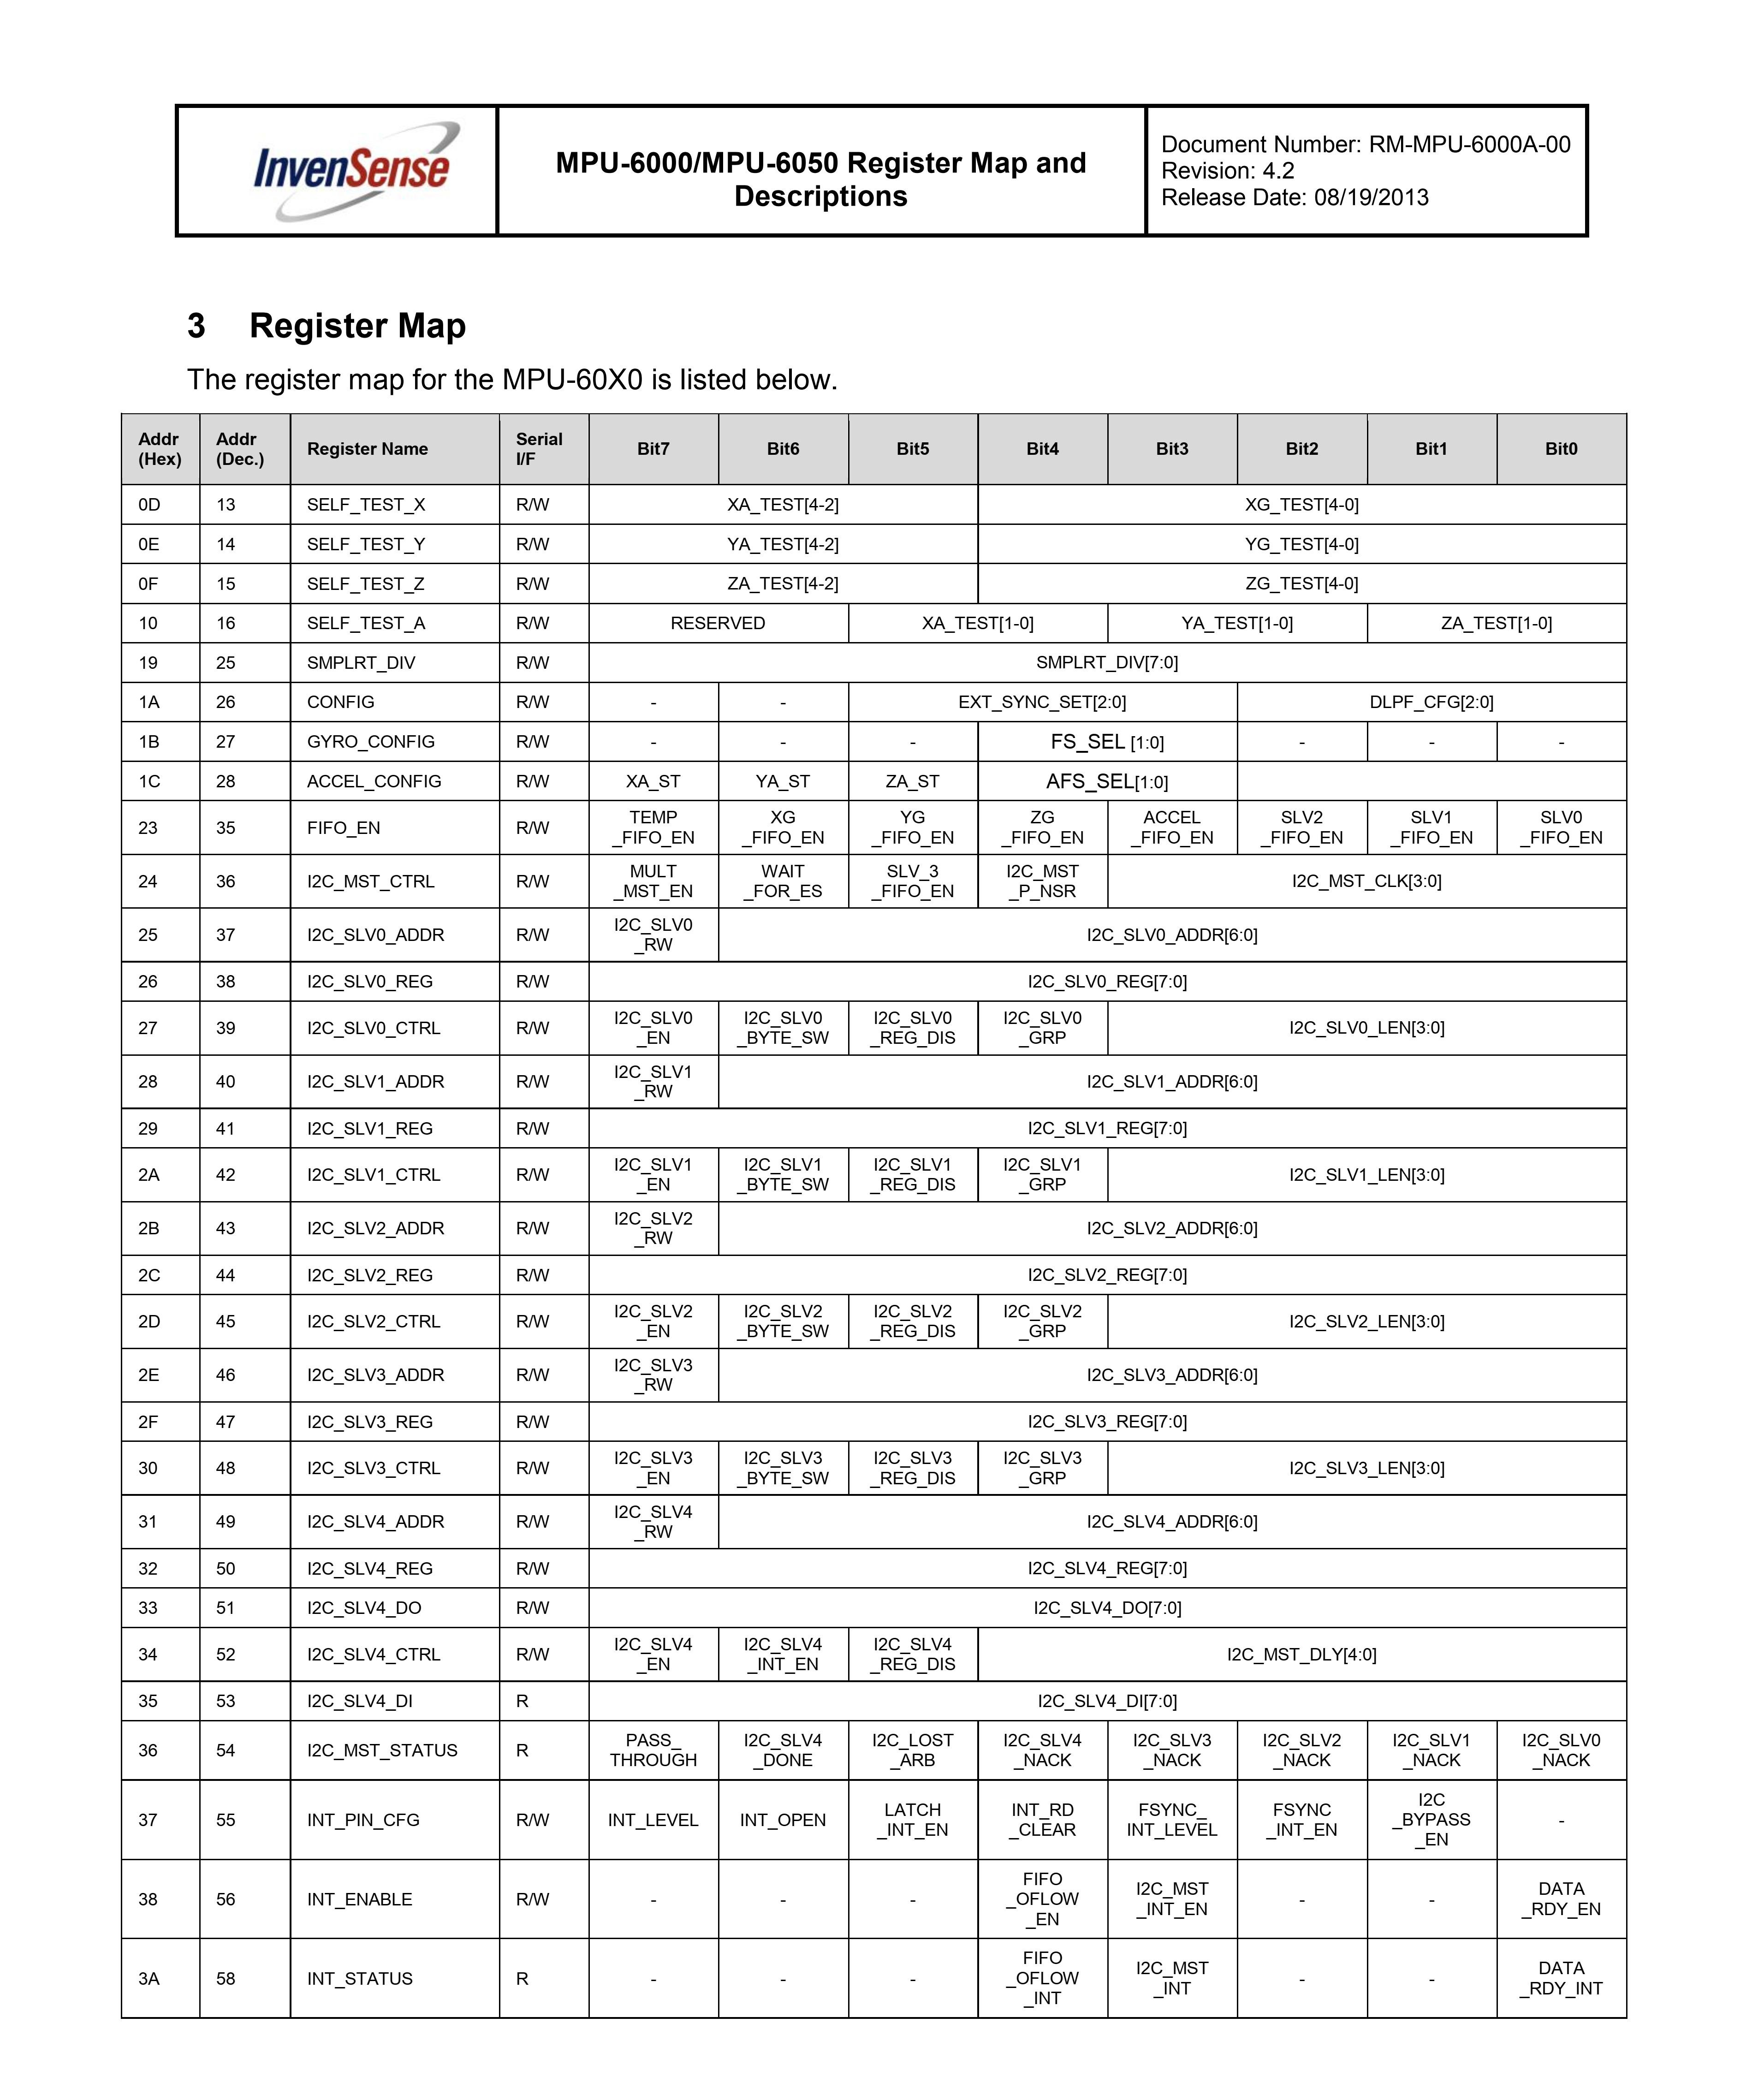
\includegraphics{5}
\end{figure} 
\begin{figure}[h!]
	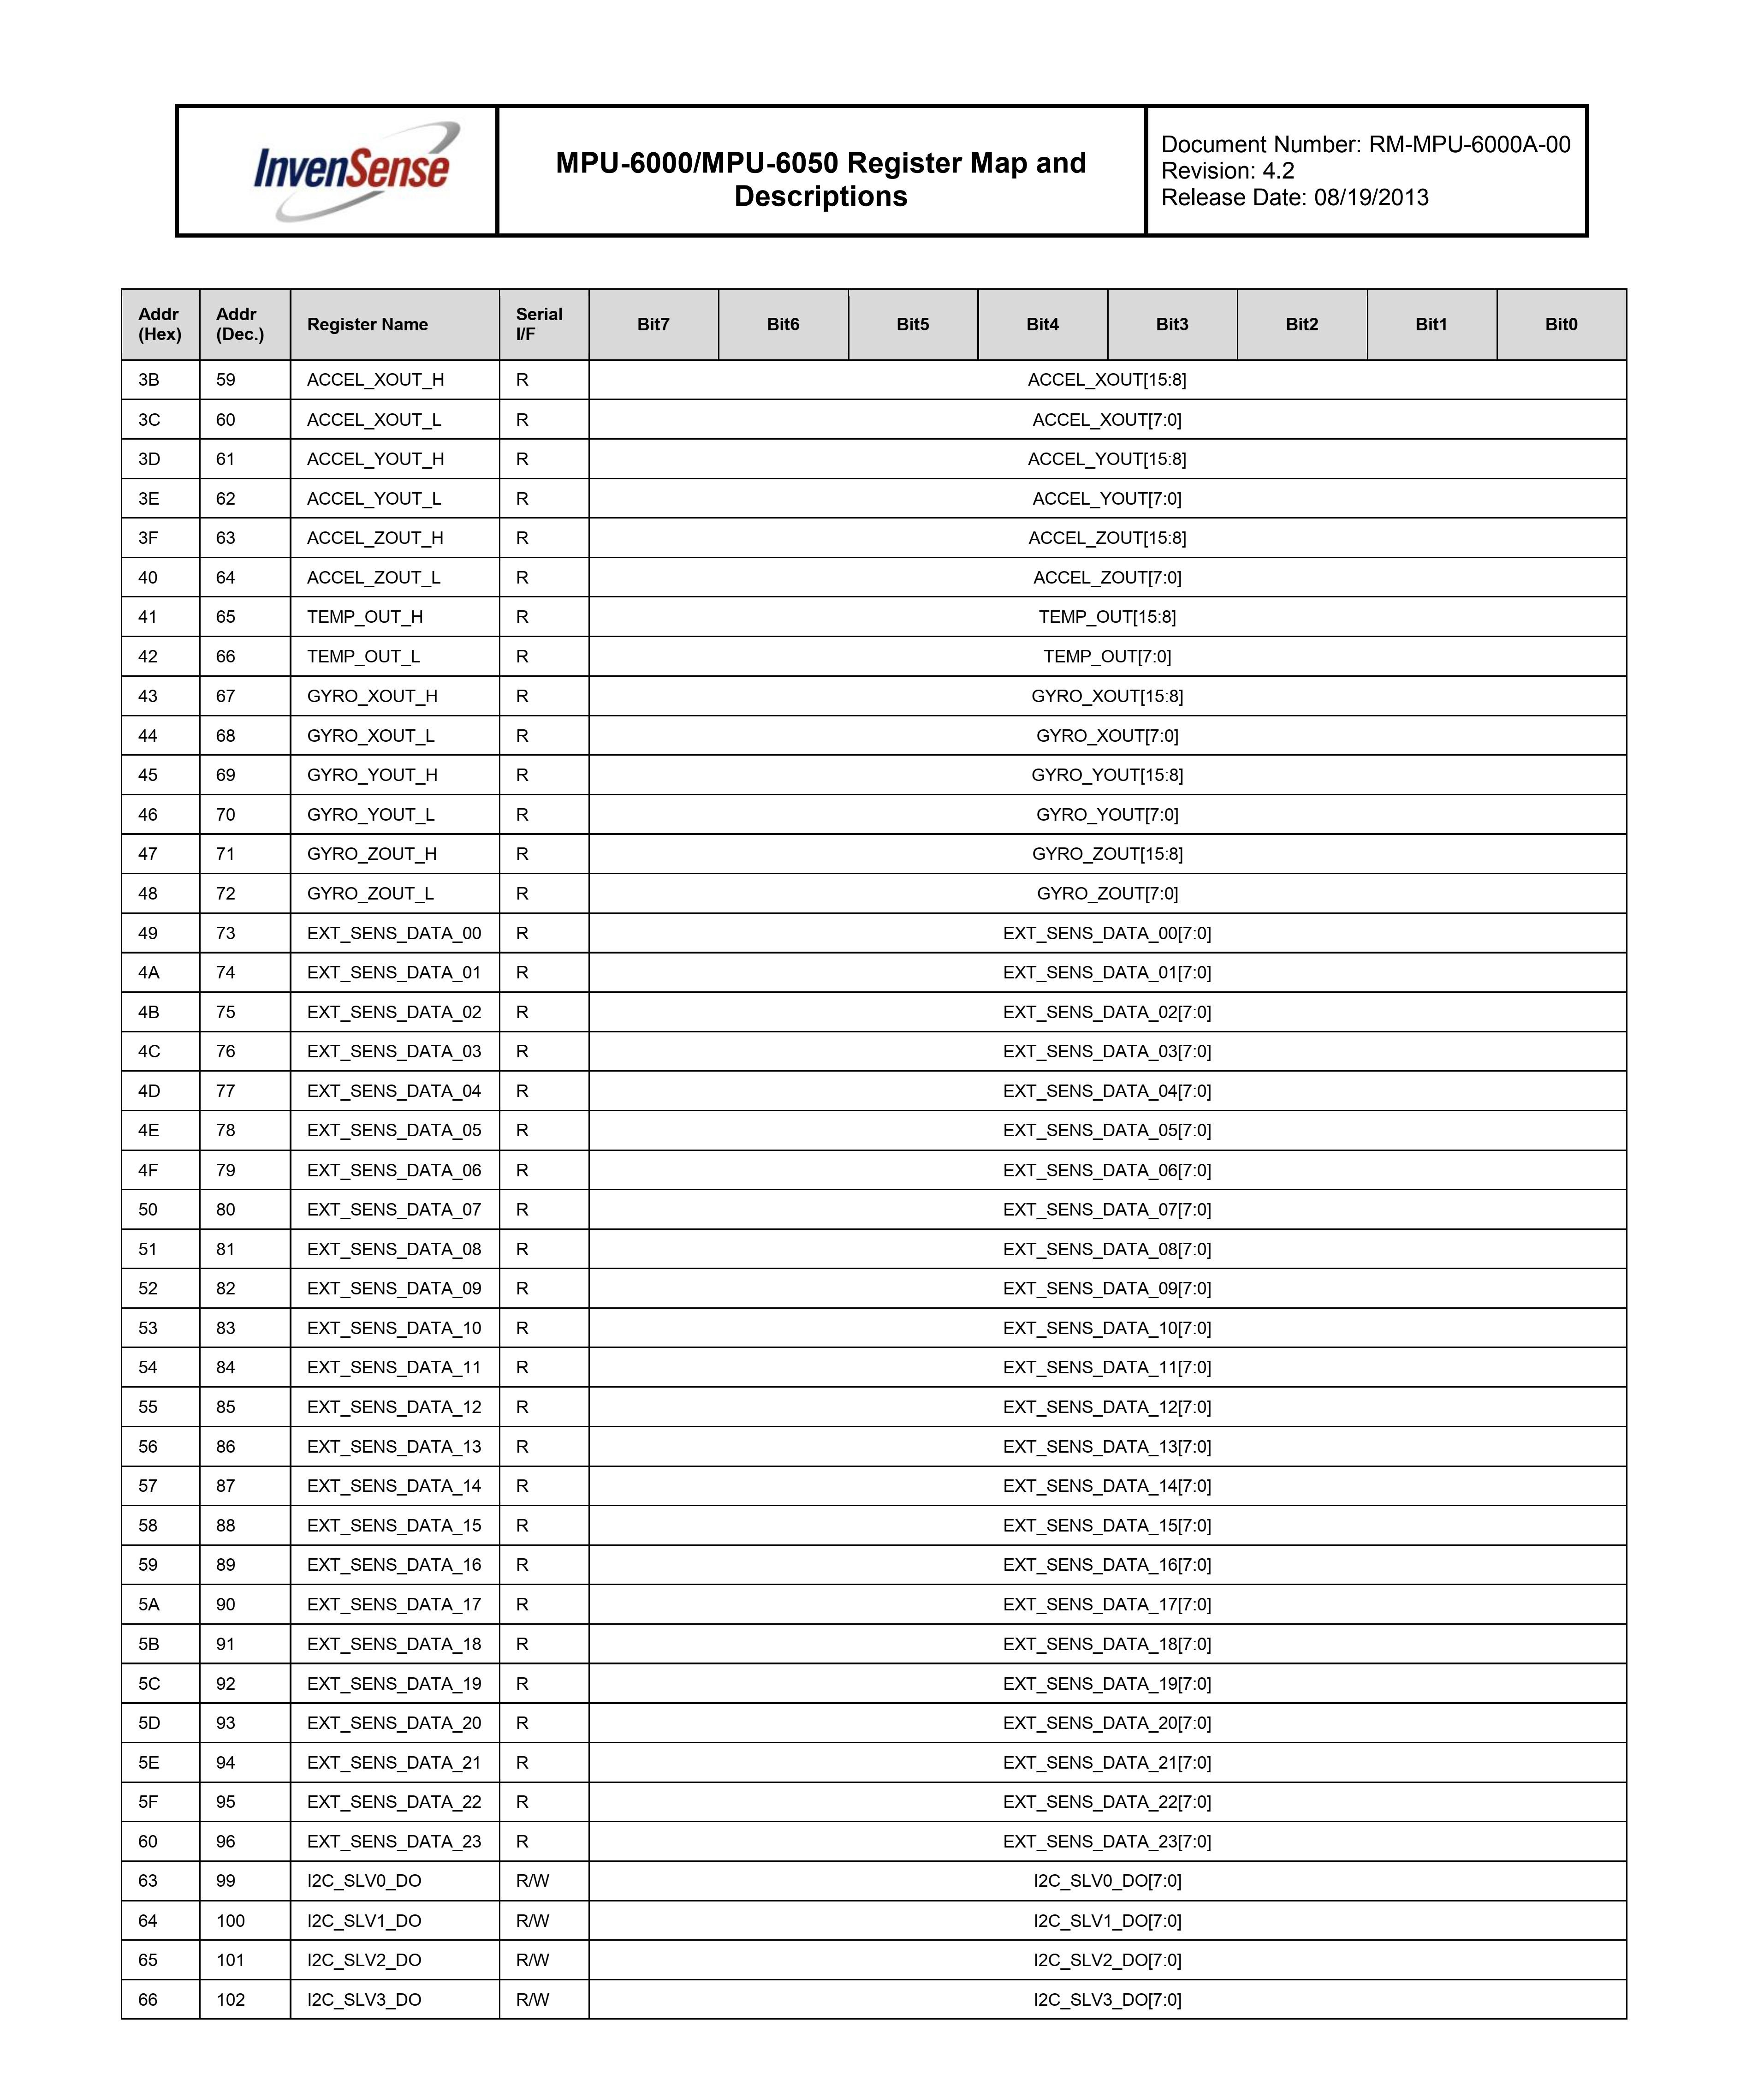
\includegraphics{6}
\end{figure}
\begin{figure}[h!]
	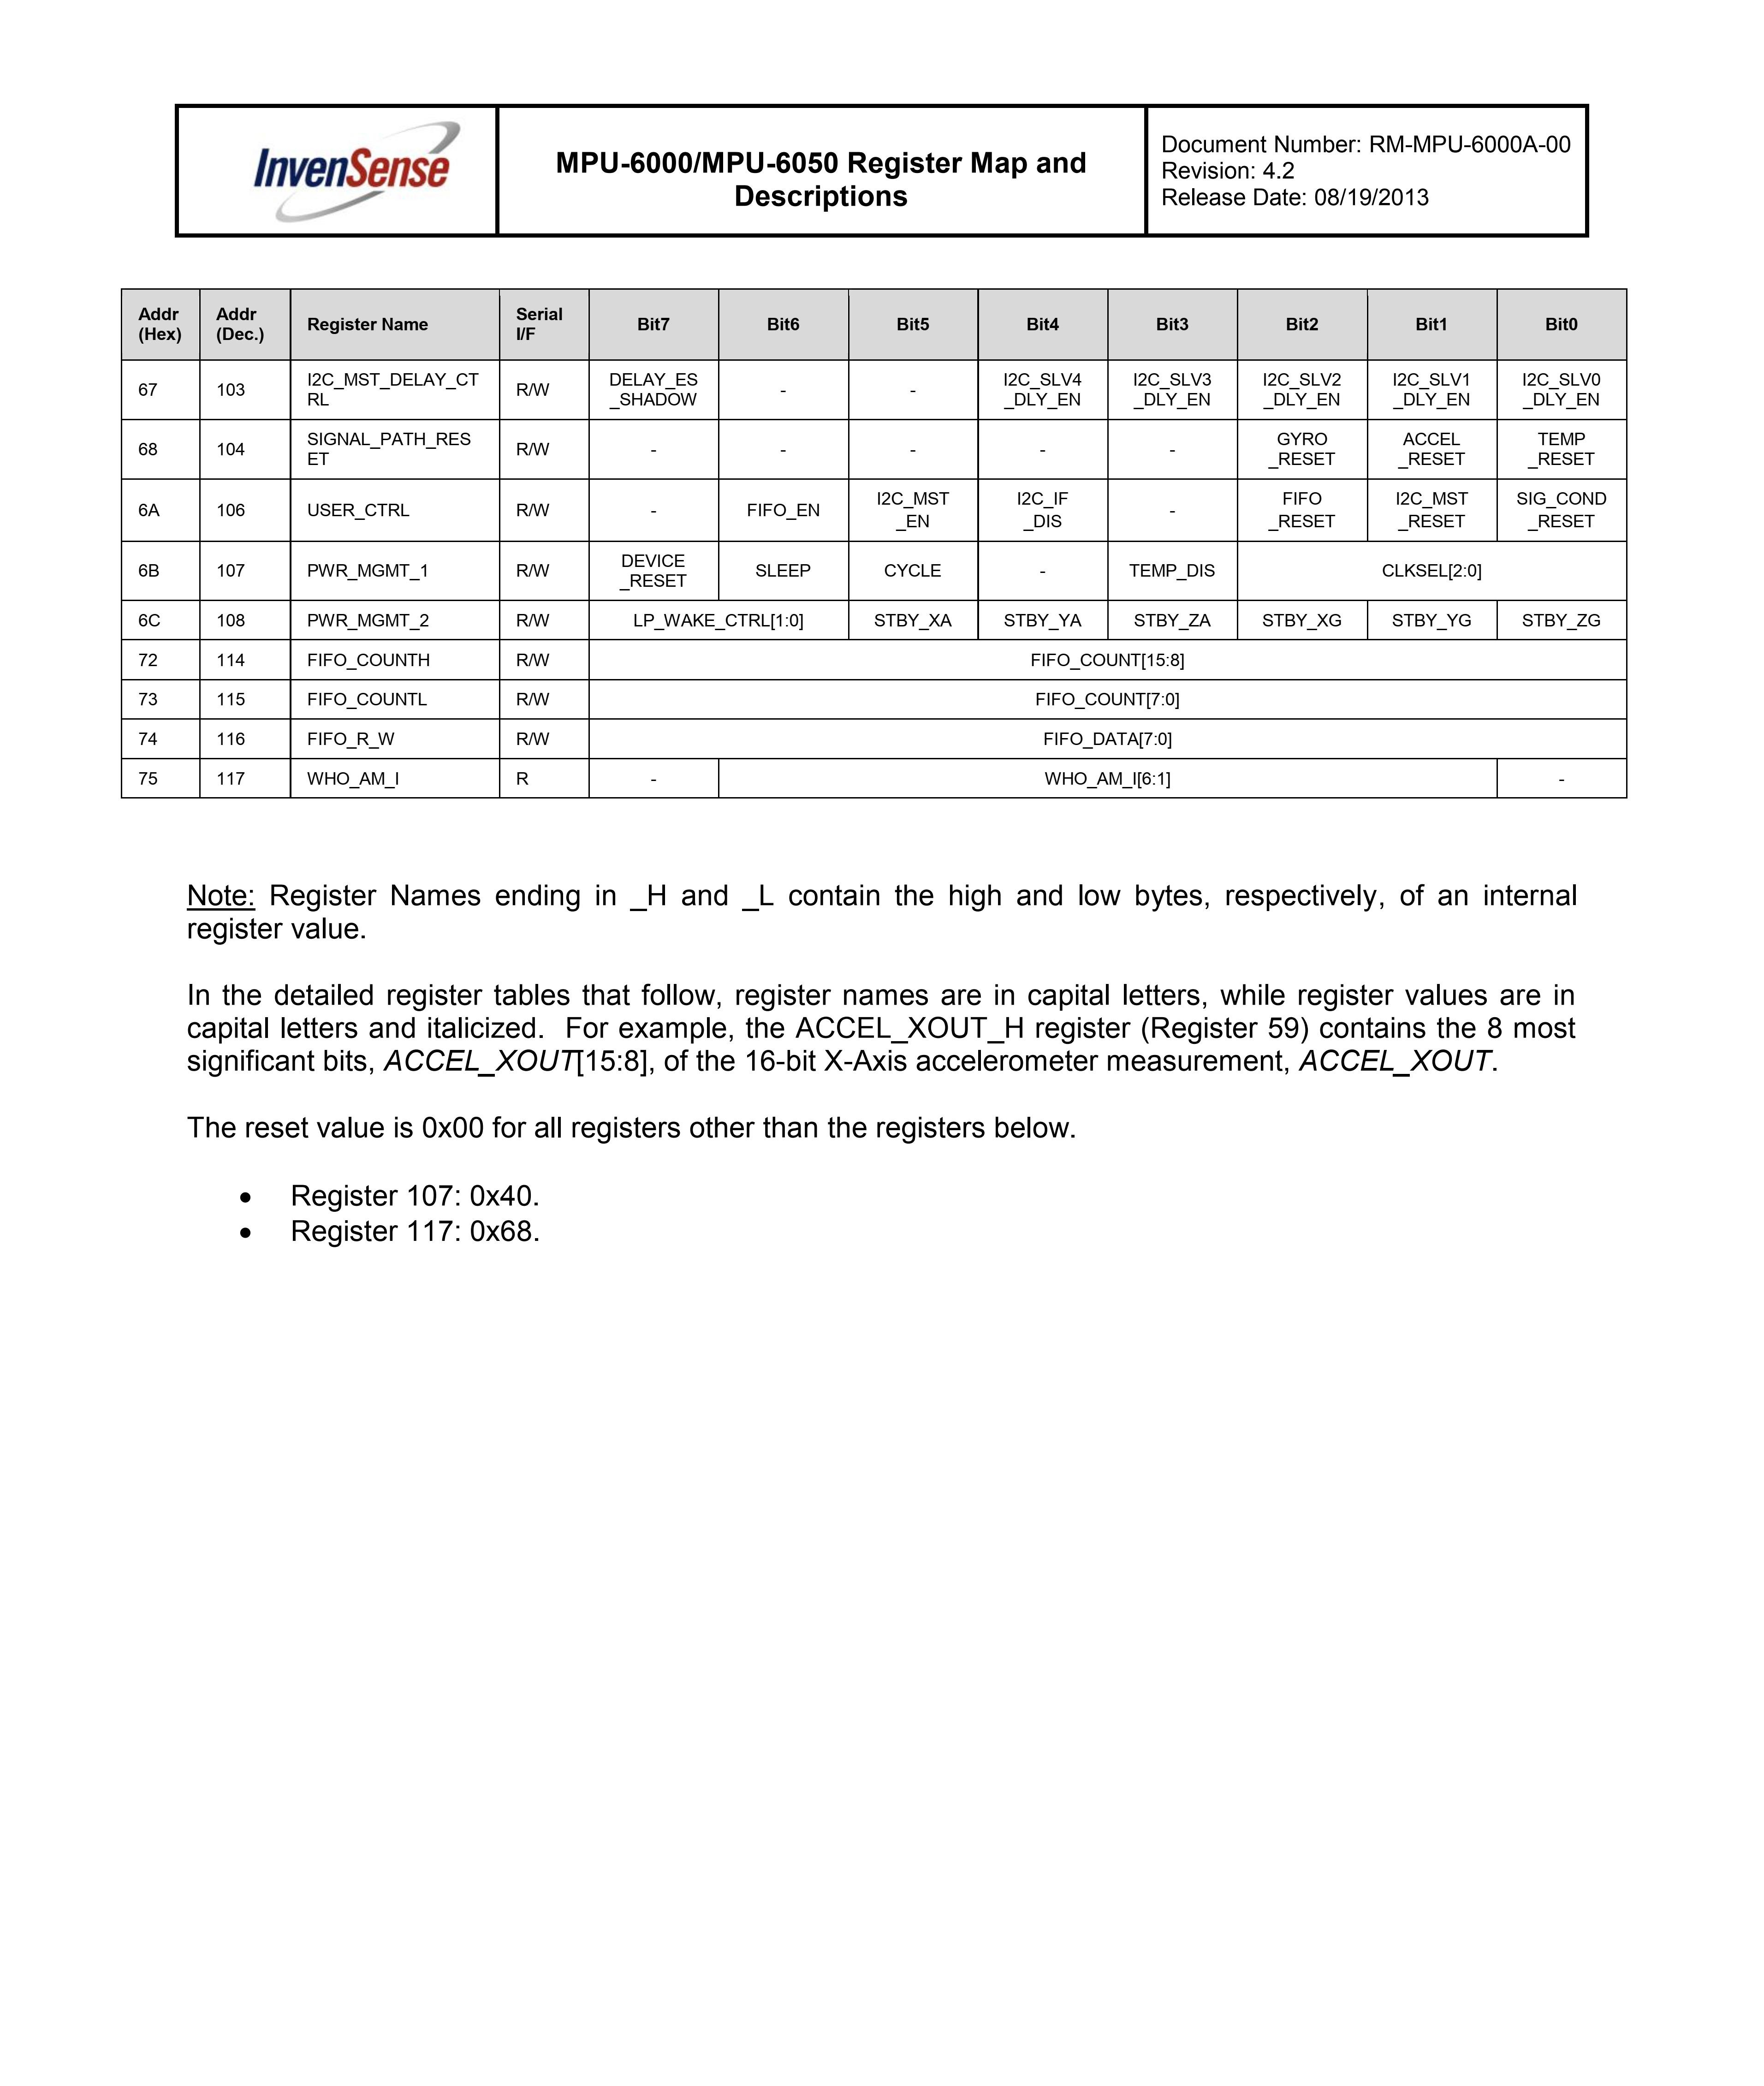
\includegraphics{7}
\end{figure}
\chapter{Python Code for Data Acquisition Program}
\begin{verbatim}
import matplotlib.pyplot as plt
import matplotlib.animation as animation
from drawnow import *
import socketserver

accel = []
gyro = []
plt.ion() #tell the matplotlib that we want to draw live data
def makeFig():
plt.subplot(2,1,1)
plt.plot(accel, 'r', label= 'Normalized Acceleration')
plt.legend(loc='upper left')
plt.ylim(0,5)
plt.subplot(2,1,2)
plt.plot(gyro, 'b', label = 'Normalized Angular Velocity')
plt.legend(loc='upper left')
plt.savefig('testplot.png')

class myTCPServer(socketserver.StreamRequestHandler):
def handle(self):
data = self.rfile.readline()
dataArray = data.decode().split(',')
normAcc = float(dataArray[0])
normGyro = float(dataArray[1])
accel.append(normAcc)
gyro.append(normGyro)
if len(accel) > 100:
accel.pop(0)
if len(gyro) > 100:
gyro.pop(0)
drawnow(makeFig)
#create TCP server
serv = socketserver.TCPServer(("",8000),myTCPServer)
serv.serve_forever()
\end{verbatim}%
%----------------------------------------------------------------------
% END MATERIAL
%----------------------------------------------------------------------

% B I B L I O G R A P H Y
% -----------------------

% The following statement selects the style to use for references.  It controls the sort order of the entries in the bibliography and also the formatting for the in-text labels.

% This specifies the location of the file containing the bibliographic information.  
% It assumes you're using BibTeX (if not, why not?).
\cleardoublepage % This is needed if the book class is used, to place the anchor in the correct page,
                 % because the bibliography will start on its own page.
                 % Use \clearpage instead if the document class uses the "oneside" argument
\phantomsection  % With hyperref package, enables hyperlinking from the table of contents to bibliography             
% The following statement causes the title "References" to be used for the bibliography section:
\renewcommand*{\bibname}{References}

% Add the References to the Table of Contents
\addcontentsline{toc}{chapter}{\textbf{References}}
\bibliographystyle{IEEEtran}
\bibliography{uw-ethesis}
% Tip 5: You can create multiple .bib files to organize your references. 
% Just list them all in the \bibliogaphy command, separated by commas (no spaces).

% The following statement causes the specified references to be added to the bibliography% even if they were not 
% cited in the text. The asterisk is a wildcard that causes all entries in the bibliographic database to be included (optional).


\end{document}
